\documentclass[12pt,a4paper]{article}

% --- Encoding and fonts ---
\usepackage[utf8]{inputenc}
\usepackage[T1]{fontenc}
\usepackage{mathpazo}

% --- Mathematics ---
\usepackage{amsmath,amssymb,amsthm,mathtools}
\usepackage{bm}

% --- Layout ---
\usepackage[margin=2.5cm]{geometry}
\usepackage{setspace}
\onehalfspacing
\usepackage{parskip}
\usepackage{microtype}
\setlength{\emergencystretch}{2.5em} % let TeX stretch spaces rather than overflow the margin

% --- Graphics and tables ---
\usepackage{graphicx}
\usepackage{booktabs}
\usepackage{multirow}
\usepackage{float}
\usepackage{caption}
\usepackage{subcaption}
\renewcommand{\topfraction}{0.85}
\renewcommand{\textfraction}{0.1}
\renewcommand{\floatpagefraction}{0.75} % a large figure goes on top of a text page rather than on a page of its own

% --- Hyperlinks ---
\usepackage[colorlinks=true,citecolor=blue,linkcolor=blue,urlcolor=blue]{hyperref}

% --- Bibliography ---
\usepackage{natbib}
\bibliographystyle{plainnat}

% --- Algorithms ---
\usepackage{algorithm}
\usepackage{algpseudocode}

% --- Theorem environments ---
\newtheorem{proposition}{Proposition}
\newtheorem{theorem}{Theorem}
\newtheorem{lemma}{Lemma}
\newtheorem{corollary}{Corollary}
\newtheorem{assumption}{Assumption}
\newtheorem{remark}{Remark}
\newtheorem{definition}{Definition}

% --- Custom commands ---
\newcommand{\E}{\mathbb{E}}
\newcommand{\Var}{\mathrm{Var}}
\newcommand{\Cov}{\mathrm{Cov}}
\newcommand{\bW}{\mathbf{W}}
\newcommand{\bX}{\mathbf{X}}
\newcommand{\bZ}{\mathbf{Z}}
\newcommand{\bH}{\mathbf{H}}
\newcommand{\by}{\mathbf{y}}
\newcommand{\bv}{\mathbf{v}}
\newcommand{\bu}{\mathbf{u}}
\newcommand{\bbeta}{\boldsymbol{\beta}}
\newcommand{\bgamma}{\boldsymbol{\gamma}}
\newcommand{\bmu}{\boldsymbol{\mu}}
\newcommand{\bpi}{\boldsymbol{\pi}}
\newcommand{\btheta}{\boldsymbol{\theta}}
\newcommand{\plim}{\overset{p}{\longrightarrow}}
\newcommand{\dlim}{\overset{d}{\longrightarrow}}
\DeclareMathOperator{\logit}{logit}
\DeclareMathOperator{\diag}{diag}
\DeclareMathOperator{\tr}{tr}

% =============================================================================
\title{ZISAR: A Zero-Inflated Spatial Autoregressive\\Model for Count Data with Random Effects}

\author{
  Niccol\`{o} Salvini\thanks{Department of Statistical Sciences, Universit\`{a} Cattolica del Sacro Cuore, Italy.}
  \and
  Giuseppe Arbia\footnotemark[1]
  \and
  Vincenzo Nardelli\footnotemark[1]
}

\date{\today}

% =============================================================================
\begin{document}

\maketitle

\begin{abstract}
Spatial count data with excess zeros arise frequently in regional science, epidemiology, and urban economics, yet the existing econometric toolkit lacks a unified frequentist framework that simultaneously addresses spatial spillovers through a structural autoregressive mechanism, zero-inflation, overdispersion, and unobserved heterogeneity.
We introduce the Zero-Inflated Spatial Autoregressive (ZISAR) model, which places a simultaneous autoregressive (SAR) structure on the latent linear predictor of a zero-inflated negative binomial specification: the log-conditional mean follows $\boldsymbol{\eta} = (\mathbf{I} - \rho\mathbf{W})^{-1}(\mathbf{X}\boldsymbol{\beta} + \mathbf{u})$, where the spatial multiplier $(\mathbf{I} - \rho\mathbf{W})^{-1}$ generates endogenous feedback effects among neighbouring units and unit-level Gaussian random effects $\mathbf{u}$ capture residual heterogeneity.
The general formulation allows a separate SAR process in the zero-inflation component, with a restricted version confining spatial dependence to the count process.
Estimation proceeds by maximising the Laplace-approximated marginal likelihood, implemented via Template Model Builder (\texttt{TMB}), which exploits automatic differentiation and sparse-matrix algebra for scalable inference.
We establish consistency and asymptotic normality of the estimator and derive closed-form expressions for direct, indirect, and total marginal effects that account for both the mixture structure and the spatial multiplier.
For large $n$, the log-determinant of the spatial filter is obtained from a sparse Cholesky factorisation, so that no dense $n\times n$ matrix is formed.
A Monte~Carlo study demonstrates that ignoring either zero-inflation or spatial dependence induces substantial bias in the autoregressive and regression coefficients, whereas ZISAR recovers the data-generating parameters with low bias and an RMSE that decreases with the sample size, and that residual-based Moran tests can miss spatial dependence that the likelihood detects.
An application to domestic solar photovoltaic installations in the 32{,}322 small areas of England after the 2016 reform of the Feed-in Tariff, where a third of the areas record no installation, estimates strong spatial dependence in the latent propensity to adopt ($\hat\rho = 0.63$), attributes about one zero in ten to the structural regime of flat-dominated urban cores, and shows that aspatial models misread the spatial clustering of adoption as effects of tenure and age.
Companion \texttt{R} code and the \texttt{TMB} template implementing the estimator are provided.

\end{abstract}

\noindent\textbf{Keywords:} Spatial autoregression; zero-inflated models; count data; negative binomial; random effects; two-step estimation; spatial spillovers; solar photovoltaic adoption.

\bigskip

\section{Introduction}\label{sec:introduction}

Count data exhibiting both spatial dependence and an excess of zeros are pervasive in the applied sciences.
Emergency-department admissions across municipalities, recorded offences across neighbourhoods, firm start-up counts by county, patent citations at the regional level, and disease incidence in small areas all share a common statistical signature: many spatial units record a zero outcome, the non-zero counts display overdispersion relative to the Poisson, and neighbouring units tend to report similar values.
Despite the empirical ubiquity of this data structure, the econometric literature has addressed its three defining features---spatial spillovers, zero-inflation, and overdispersion---largely in isolation or in pairwise combinations, leaving a methodological gap that this paper aims to fill.

In the spatial econometrics tradition initiated by \citet{anselin1988} and surveyed comprehensively by \citet{lesage_pace2009} and \citet{arbia2006,arbia2024}, the workhorse specification for modelling cross-sectional dependence is the spatial autoregressive (SAR) model $\by = \rho\bW\by + \bX\bbeta + \varepsilon$, where $\bW$ is a row-standardised spatial weights matrix and $\rho$ captures endogenous interaction effects among neighbouring units.
For continuous outcomes, maximum-likelihood and generalised-method-of-moments estimators are well established \citep{lee2004,kelejian_prucha1998,kelejian_prucha1999}.
Extending the SAR logic to count data is substantially more challenging because the conditional mean is linked to the linear predictor through a nonlinear (log or exponential) function, and the endogeneity of $\bW\by$ interacts with the discreteness of the support.
\citet{lambert2010} proposed a two-step limited-information maximum likelihood (LIML) estimator for a spatial lag Poisson model, providing a structurally consistent framework that has since become the main reference for SAR-type count models.
However, the Lambert--Brown--Florax estimator handles neither zero-inflation nor overdispersion, two phenomena that routinely co-occur in spatial count data.

On a separate track, the zero-inflated Poisson (ZIP) and zero-inflated negative binomial (ZINB) models, pioneered by \citet{lambert1992} and studied extensively by \citet{cameron_trivedi2013} and \citet{hilbe2011}, accommodate excess zeros through a two-component mixture: a degenerate point mass at zero (the ``structural'' or ``inflation'' component) and a standard count distribution (the ``count'' or ``sampling'' component).
These models have become standard in biostatistics and health economics but, in their classical form, assume independence across observations.
When applied to spatially referenced data, the residuals typically exhibit positive autocorrelation, leading to efficiency losses and potentially biased inference on covariate effects \citep{arbia2006}.

Attempts to marry zero-inflation with spatial structure have taken two main routes.
The spatial-statistics approach introduces conditionally autoregressive (CAR) or geostatistical random effects into one or both components of the ZIP/ZINB model, typically within a Bayesian framework.
Notable examples include the \texttt{CARBayes} package of \citet{lee2013}, the INLA-based disease-mapping models of \citet{asmarian2019}, and the spatial Poisson hurdle specification of \citet{neelon2013}.
While these methods elegantly capture residual spatial heterogeneity, they model dependence as a latent effect rather than as a structural, endogenous interaction.
Consequently, they cannot identify or quantify the direct and indirect (spillover) effects that are central to the spatial econometrics programme \citep{lesage_pace2009,lesage_pace2014}.
The spatial-filtering approach of \citet{metulini2018} and \citet{griffith2003} offers an intermediate solution by projecting spatial dependence onto a set of Moran eigenvectors included as regressors in a standard ZIP/ZINB; this avoids the endogeneity problem but sacrifices the structural interpretation of $\rho$ as a measure of spatial contagion.

No existing framework unifies all four desiderata---endogenous spatial lag, zero-inflation, overdispersion, and unobserved unit-level heterogeneity---within a single, frequentist, estimable specification.
This paper introduces the \emph{Zero-Inflated Spatial Autoregressive} (ZISAR) model to close this gap.
Our contributions are four.
First, we propose a zero-inflated negative binomial model in which the latent linear predictor of the count process follows a simultaneous autoregressive structure: $\boldsymbol{\eta} = (\mathbf{I} - \rho\bW)^{-1}(\bX\bbeta + \bu)$, where the spatial multiplier $(\mathbf{I} - \rho\bW)^{-1}$ propagates covariate effects across the spatial network and unit-level Gaussian random effects $\bu$ capture residual heterogeneity.
The general specification allows a separate SAR process in the zero-inflation component, estimated through a reduced-rank field on a lattice of knots; a restricted version confines spatial dependence to the count predictor.
The model nests several important special cases: setting $\rho=0$ recovers the standard ZINB with random effects; removing random effects and zero-inflation collapses to the aspatial Poisson.

Second, the SAR-on-$\boldsymbol{\eta}$ formulation avoids the endogeneity of observed spatial lags that plagues SAR-on-$\by$ specifications \citep{lambert2010}, enabling proper maximum-likelihood estimation.
We maximise the Laplace-approximated marginal likelihood via Template Model Builder \citep[\texttt{TMB};][]{kristensen2016}, which exploits automatic differentiation and sparse-matrix algebra to scale to $n = O(10^4)$.
This estimation strategy shares the scalability concerns of \citet{arbia_nardelli2024} while delivering exact (up to the Laplace order) marginal inference.

Third, we establish the consistency and asymptotic normality of the Laplace-approximate MLE under regularity conditions analogous to those in \citet{lee2004} and \citet{newey_mcfadden1994}, and derive closed-form expressions for direct, indirect, and total marginal effects that account for both the zero-inflation mixture and the spatial multiplier, adapting the \citet{lesage_pace2009} framework to the nonlinear ZINB setting.

Fourth, we release the estimator, the effects decomposition and prediction in the open-source \texttt{R} package \texttt{zisar} \citep{zisar_pkg}, and demonstrate the model on a Monte~Carlo study and on an application to the $32{,}322$ small areas of England, which the sparse log-determinant of Section~\ref{sec:est_laplace} makes feasible at full scale.
In the adoption of domestic solar photovoltaic systems during the boom of the Feed-in Tariff both parts of the restricted model are needed---spatial dependence in the counts and structural zeros where the housing stock leaves no roofs to equip---and the effects decomposition attributes the larger part of every total effect to spillovers.

The remainder of the paper is organised as follows.
Section~\ref{sec:literature} surveys the existing literature on spatial count models, zero-inflated spatial specifications, and spatial filtering approaches.
Section~\ref{sec:model} introduces the ZISAR model and states its key properties.
Section~\ref{sec:estimation} details the Laplace-approximate ML procedure and derives the asymptotic results and effects decomposition.
Section~\ref{sec:montecarlo} reports a Monte~Carlo study comparing ZISAR with competing specifications and the power of tests for spatial dependence.
Section~\ref{sec:solar} applies the restricted model to the adoption of domestic solar photovoltaic systems in the small areas of England during the boom of the Feed-in Tariff and reports its direct and indirect effects.
Section~\ref{sec:conclusion} concludes and discusses extensions, including the incorporation of temporal dependence.
Proofs, the simulation checks of the general model and implementation details are collected in the Appendix.


\section{Literature Review}\label{sec:literature}

The challenge of modelling spatially dependent count data with excess zeros sits at the intersection of three well-developed but largely separate literatures: spatial econometrics for count data, zero-inflated models with spatial latent effects, and spatial filtering approaches.
We review each stream in turn, highlighting the strengths and limitations that motivate the ZISAR specification.

% ---------------------------------------------------------------------------
\subsection{Spatial autoregressive models for count data}\label{sec:lit_sar_count}

The foundation of spatial econometrics rests on the SAR (spatial autoregressive or spatial lag) model, which captures endogenous interaction effects through the term $\rho\bW\by$ \citep{anselin1988,lesage_pace2009}.
For continuous outcomes, \citet{lee2004} established the asymptotic theory for quasi-maximum-likelihood estimation, while \citet{kelejian_prucha1998,kelejian_prucha1999} developed GMM alternatives.
The theoretical and applied foundations of these methods are extensively treated in \citet{arbia2006} and \citet{arbia2024}, who provide a rigorous statistical grounding for spatial interaction models and their implementation in modern software environments.

Extending the SAR paradigm to discrete, non-negative outcomes is non-trivial.
The fundamental difficulty is that the spatial multiplier $(I - \rho\bW)^{-1}$, which in the linear-Gaussian case yields a closed-form reduced form, does not interact gracefully with the exponential link function inherent in Poisson and negative binomial models.
\citet{lambert2010} addressed this by proposing a two-step LIML estimator for a spatial lag Poisson specification.
Their approach instruments the endogenous $\bW\by$ with its projection onto the space spanned by exogenous regressors and their spatial lags, $(\bX, \bW\bX, \bW^2\bX)$, and then maximises the Poisson log-likelihood evaluated at the fitted instruments.
Monte~Carlo evidence showed that the estimator achieves substantial bias reductions compared to a na\"{\i}ve aspatial Poisson, particularly as $\rho$ and $n$ grow.
\citet{sellner2013} applied a similar logic to gravity models of trade, estimating a spatial autoregressive Poisson gravity specification.

\citet{glaser2017} provided a comprehensive review of spatial econometric models for count data, classifying existing approaches by how they introduce spatial structure (lag, error, or Durbin), which count distribution they assume, and how they handle estimation.
A recurring theme is that most implementations remain limited to the Poisson distribution and do not accommodate excess zeros or overdispersion---two features that pervade empirical spatial count datasets.
As \citet{cameron_trivedi2013} note in the non-spatial context, the Poisson's equidispersion restriction ($\E[y_i] = \Var[y_i]$) is almost always violated in practice, and failure to account for overdispersion inflates test sizes and narrows confidence intervals.

The pairwise pseudo-likelihood methods developed by \citet{arbia_nardelli_salvini} and \citet{arbia_nardelli2024} offer a parallel advance in making spatial estimation feasible for large and irregular lattices.
Their sampled-grid and KD-tree algorithms reduce the $O(n^3)$ bottleneck of full likelihood to near-linear cost while retaining consistency, a property that is especially valuable when the spatial weights matrix is dense or the sample size is large.
While these methods were developed for Gaussian spatial models, the underlying principle---replacing the full likelihood with a computationally tractable surrogate that preserves consistency---resonates with the instrumental-variables philosophy we adopt for the ZISAR estimator.

% ---------------------------------------------------------------------------
\subsection{Zero-inflated spatial models with latent effects}\label{sec:lit_zi_spatial}

A second body of literature models spatial dependence in zero-inflated counts not through an endogenous lag $\bW\by$ but through spatially structured random effects, typically within a Bayesian hierarchical framework.

The zero-inflated Poisson (ZIP) model \citep{lambert1992} and its negative binomial extension (ZINB) \citep{cameron_trivedi2013,hilbe2011} decompose the observed count into a degenerate component (``structural zeros'') and a count component, governed respectively by a Bernoulli and a Poisson or NB process.
In the non-spatial setting, these models are well understood and widely implemented \citep[e.g.][]{zeileis2008,brooks2017}.
When observations are georeferenced, however, residual spatial autocorrelation in one or both components can bias covariate effects and distort inference.

The standard spatial-statistical remedy is to augment the linear predictor with conditionally autoregressive (CAR) random effects \citep{besag_york_mollie1991}.
\citet{lee2013} implemented this strategy in the \texttt{CARBayes} package for \texttt{R}, which supports Poisson, ZIP, and NB likelihoods with Leroux-type CAR priors, estimated via MCMC.
In the disease-mapping literature, \citet{asmarian2019} combined zero-inflated specifications with BYM (Besag--York--Molli\'{e}) random effects and estimated the resulting model through integrated nested Laplace approximations (INLA) \citep{rue_martino_chopin2009}, demonstrating good performance on Iranian cancer-registry data.
\citet{he2024} pushed this line further by replacing the discrete CAR specification with a nearest-neighbour Gaussian process (NNGP), achieving scalability to tens of thousands of spatial locations within a Bayesian ZINB framework.

\citet{neelon2013} developed a spatial Poisson hurdle model for emergency-department visit data---an application closely related to ours---with bivariate CAR priors linking the hurdle and count components.
Their model, published in this journal, demonstrated that ignoring spatial structure in the analysis of ED utilisation leads to attenuated covariate effects and misleading maps of geographic variation.

While these Bayesian spatial ZI models are flexible and increasingly scalable, they differ from the ZISAR approach in a fundamental way: the spatial dependence operates through latent random effects rather than through the observed outcome $\by$.
As a consequence, the fitted models do not yield the \emph{direct} and \emph{indirect effects} decomposition of \citet{lesage_pace2009} that is central to the spatial econometrics programme.
The distinction is not merely taxonomic.
When $\bW\by$ enters the conditional mean directly, a change in a covariate in region $j$ affects the outcome in region $i$ not only through region $j$'s own count but also through the spatial multiplier $(I - \rho\bW)^{-1}$, generating a cascade of feedback effects whose magnitude depends on the network topology.
CAR-based models, by contrast, attribute all cross-regional correlation to unobserved confounders, precluding any structural interpretation of spillovers.

% ---------------------------------------------------------------------------
\subsection{Spatial filtering with zero-inflated counts}\label{sec:lit_esf}

A third approach avoids the endogeneity issue altogether by projecting the spatial autocorrelation structure onto a set of synthetic regressors derived from the eigenvectors of a transformed spatial weights matrix.
\citet{griffith2003} laid the theoretical foundations for eigenvector spatial filtering (ESF), showing that a judiciously chosen subset of Moran eigenvectors can absorb spatial autocorrelation from the residuals of a GLM.
\citet{griffith_chun2014} extended the framework and provided practical guidance for eigenvector selection.

\citet{metulini2018} applied ESF to a zero-inflated gravity model of trade, demonstrating that including Moran eigenvectors in both the inflation and count components of a ZIP effectively removes spatial residual autocorrelation without introducing endogeneity.
Their Monte~Carlo evidence showed that the spatial-filtering ZIP outperforms the standard ZIP in terms of bias and coverage when the data-generating process exhibits spatial dependence.

The appeal of ESF lies in its computational simplicity---once the eigenvectors are computed, the model reduces to a standard GLM---and in its compatibility with any count distribution, including ZIP and ZINB.
The trade-off is interpretive: the eigenvector coefficients do not map onto a single, economically meaningful parameter such as $\rho$, making it difficult to quantify the strength and reach of spatial spillovers.
Moreover, the choice of which and how many eigenvectors to include introduces a model-selection step that can be sensitive to the criterion employed \citep{griffith_chun2014}.

% ---------------------------------------------------------------------------
\subsection{Positioning the ZISAR model}\label{sec:lit_gap}

Table~\ref{tab:litgap} summarises the features addressed by each strand of the literature.
The key observation is that no existing specification simultaneously accommodates an endogenous spatial lag, zero-inflation, overdispersion (NB), and unit-level random effects in a frequentist framework amenable to direct/indirect effects decomposition.

\begin{table}[htbp]
\centering
\caption{Features of existing spatial count models and the proposed ZISAR.}\label{tab:litgap}
\small
\begin{tabular}{lccccc}
\toprule
Specification & SAR lag & Zero-infl. & NB & Random eff. & Direct/indirect \\
\midrule
SAR-Poisson \citep{lambert2010}        & \checkmark & -- & -- & -- & \checkmark \\
SAR-Poisson gravity \citep{sellner2013} & \checkmark & -- & -- & -- & \checkmark \\
ZINB \citep{cameron_trivedi2013}        & -- & \checkmark & \checkmark & -- & -- \\
ZIP + CAR \citep{lee2013}               & -- & \checkmark & -- & CAR & -- \\
ZIP hurdle + CAR \citep{neelon2013}     & -- & \checkmark & -- & CAR & -- \\
ZINB + NNGP \citep{he2024}             & -- & \checkmark & \checkmark & GP & -- \\
ZIP + ESF \citep{metulini2018}          & (proxy) & \checkmark & -- & -- & -- \\
\midrule
\textbf{ZISAR (this paper)}             & \checkmark & \checkmark & \checkmark & unit-level & \checkmark \\
\bottomrule
\end{tabular}
\end{table}

The ZISAR model fills this gap by placing a simultaneous autoregressive structure on the latent predictor of a zero-inflated NB specification, optionally extending the spatial interaction to the inflation process, and incorporating unit-level random effects for residual heterogeneity.
Unlike \citet{lambert2010}, who require instrumental variables to handle the endogeneity of $\bW\by$, the SAR-on-$\boldsymbol{\eta}$ formulation enables proper maximum-likelihood estimation via Laplace approximation \citep{kristensen2016}, sharing the scalability concerns of \citet{arbia_nardelli2024} while delivering exact marginal inference.
The effects-decomposition framework builds on \citet{lesage_pace2009} adapted to the nonlinear ZI mixture.


\section{The ZISAR Model}\label{sec:model}

% ---------------------------------------------------------------------------
\subsection{Notation and setup}\label{sec:model_notation}

Consider $n$ spatial units indexed by $i = 1,\ldots,n$, each associated with a non-negative integer outcome $y_i \in \{0,1,2,\ldots\}$.
Let $\bW = (w_{ij})_{n \times n}$ be a known, row-standardised spatial weights matrix with $w_{ii}=0$ for all $i$; typical choices include queen or rook contiguity on a regular lattice, or $k$-nearest-neighbour graphs on irregular point patterns \citep{anselin1988,arbia2006}.
Each unit is endowed with a $(p \times 1)$ vector of exogenous covariates $\mathbf{x}_i$ entering the count process and a $(q \times 1)$ vector $\mathbf{z}_i$ entering the zero-inflation process (with $\mathbf{z}_i$ possibly overlapping with or equal to $\mathbf{x}_i$).
Stacking observations, we write $\by = (y_1,\ldots,y_n)'$, $\bX = (\mathbf{x}_1,\ldots,\mathbf{x}_n)'$, and $\bZ = (\mathbf{z}_1,\ldots,\mathbf{z}_n)'$.
Let $\lambda_1 \geq \ldots \geq \lambda_n$ denote the eigenvalues of $\bW$.

% ---------------------------------------------------------------------------
\subsection{Model specification}\label{sec:model_spec}

The Zero-Inflated Spatial Autoregressive (ZISAR) model posits that each observation $y_i$ is drawn from a two-component mixture:
\begin{equation}\label{eq:mixture}
  y_i \sim
  \begin{cases}
    0 & \text{with probability } \pi_i, \\
    \mathrm{NB}(\mu_i, \kappa) & \text{with probability } 1-\pi_i,
  \end{cases}
\end{equation}
where $\mathrm{NB}(\mu_i,\kappa)$ denotes the negative binomial distribution with conditional mean $\mu_i > 0$ and shape parameter $\kappa > 0$, so that $\Var[y_i \mid s_i=0] = \mu_i + \mu_i^2/\kappa$.
The probability $\pi_i \in (0,1)$ governs the zero-inflation (or ``structural zero'') mechanism.

The defining feature of ZISAR---what distinguishes it from standard zero-inflated models and from CAR-based spatial alternatives---is that the conditional mean of the count process is governed by a \emph{latent spatial autoregressive field}.

\paragraph{Count process: SAR on the latent predictor.}
Define the latent linear predictor $\boldsymbol{\eta} = (\eta_1,\ldots,\eta_n)'$ through the simultaneous autoregressive system
\begin{equation}\label{eq:sar_eta}
  \boldsymbol{\eta} = \rho\,\bW\boldsymbol{\eta} + \bX\bbeta + \bu, \qquad \bu \sim N(\mathbf{0},\,\sigma^2\mathbf{I}_n),
\end{equation}
which yields the reduced form
\begin{equation}\label{eq:reduced_form}
  \boldsymbol{\eta} = (\mathbf{I}_n - \rho\,\bW)^{-1}(\bX\bbeta + \bu) = \mathbf{S}(\rho)\,(\bX\bbeta + \bu),
\end{equation}
where $\mathbf{S}(\rho) \equiv (\mathbf{I}_n - \rho\,\bW)^{-1}$ is the \emph{spatial multiplier matrix}.
The conditional mean of the count process is then
\begin{equation}\label{eq:count_mean}
  \mu_i = \exp(\eta_i), \qquad i = 1,\ldots,n.
\end{equation}

The scalar parameter $\rho$ governs the strength and range of spatial interaction: a change in $\bX\bbeta$ in unit $j$ propagates to $\eta_i$ for all $i$ through the power-series expansion
\begin{equation}\label{eq:power_series}
  \mathbf{S}(\rho) = \sum_{s=0}^{\infty} \rho^s\,\bW^s,
\end{equation}
which converges for $|\rho| < 1/\max(|\lambda_1|,|\lambda_n|)$.
The random effect $u_i$ captures unit-specific unobserved heterogeneity in the count intensity, and is absorbed by the spatial multiplier: the implied covariance of $\boldsymbol{\eta}$ is
\begin{equation}\label{eq:cov_eta}
  \Var[\boldsymbol{\eta}] = \sigma^2\,\mathbf{S}(\rho)\,\mathbf{S}(\rho)' = \sigma^2\bigl[(\mathbf{I}_n-\rho\bW)'(\mathbf{I}_n-\rho\bW)\bigr]^{-1},
\end{equation}
a simultaneous autoregressive covariance structure \citep{anselin1988} that should be contrasted with the conditional autoregressive (CAR) specification used in disease-mapping models \citep{besag_york_mollie1991,lee2013}.

\begin{remark}[SAR on $\boldsymbol{\eta}$ versus SAR on $\by$]\label{rem:sar_eta_vs_y}
An alternative specification places the spatial lag on the observed count: $\log(\mu_i) = \mathbf{x}_i'\bbeta + \rho\sum_j w_{ij}y_j + v_i$.
While this ``SAR-on-$\by$'' formulation has a direct contagion interpretation, it introduces endogeneity---$y_j$ is simultaneously an outcome and a regressor---requiring instrumental-variable workarounds \citep{lambert2010}.
The SAR-on-$\boldsymbol{\eta}$ formulation \eqref{eq:sar_eta} avoids this: the spatial multiplier operates on the \emph{latent} predictor, not on the observed count, enabling proper maximum-likelihood estimation without instruments.
Crucially, the spatial econometrics interpretation is preserved: $\mathbf{S}(\rho)$ generates the same direct/indirect/total effects decomposition as in the linear SAR \citep{lesage_pace2009}.
\end{remark}

\paragraph{Zero-inflation process.}
The structural-zero mechanism is governed by a latent Bernoulli indicator $s_i \sim \text{Bernoulli}(\pi_i)$, with
\begin{equation}\label{eq:zeroinfl_general}
  \logit(\pi_i) = \mathbf{z}_i'\bgamma + g_i.
\end{equation}
In the \emph{general ZISAR}, the spatial field $\mathbf{g} = (g_1,\ldots,g_n)'$ follows a separate SAR process:
\begin{equation}\label{eq:sar_g}
  \mathbf{g} = \rho_0\,\bW\mathbf{g} + \boldsymbol{\varepsilon}_0, \qquad \boldsymbol{\varepsilon}_0 \sim N(\mathbf{0},\,\sigma_0^2\mathbf{I}_n),
\end{equation}
yielding $\mathbf{g} = (\mathbf{I}_n - \rho_0\bW)^{-1}\boldsymbol{\varepsilon}_0$ with its own autoregressive parameter $\rho_0$.
This allows spatial clustering of the zero-inflation regime---for instance, neighbouring municipalities may all lack demand for a specific health service, and this absence is itself spatially structured.

\paragraph{Reduced-rank inflation field.}
A field with one element per unit is the natural specification, but each $g_i$ is informed by a single outcome that is zero or not, and Section~\ref{sec:est_laplace} shows that the Laplace approximation to its likelihood fails.
We therefore also consider a field of lower dimension,
\begin{equation}\label{eq:rr_g}
  \mathbf{g} = \mathbf{B}\boldsymbol{\alpha}, \qquad
  \boldsymbol{\alpha} = \rho_0\,\bW_K\boldsymbol{\alpha} + \boldsymbol{\varepsilon}_0, \qquad
  \boldsymbol{\varepsilon}_0 \sim N(\mathbf{0},\,\sigma_0^2\mathbf{I}_K),
\end{equation}
where $\boldsymbol{\alpha}$ holds $K \ll n$ values at the knots of a regular lattice laid over the study region, $\bW_K$ is the row-standardised contiguity matrix of the knots and $\mathbf{B}$ is an $n\times K$ matrix of local basis functions: entry $(i,k)$ is the bisquare function $(1 - d_{ik}^2/r^2)^2$ of the distance $d_{ik}$ between unit $i$ and knot $k$, zero beyond a radius $r$, and the rows are normalised to sum to one, so that $g_i$ is a weighted mean of the knot values around unit $i$ \citep{cressie_johannesson2008}.
Each knot value is informed by all the units within $r$ of the knot---some 150 in the simulations of Appendix~\ref{app:general}, with knots 10~km apart and $r = 15$~km---and the field is smooth at scales below the knot spacing.
The parameters are those of the general model, $\rho_0$ and $\sigma_0^2$, now describing the process at the knots, with $\rho_0 \ge 0$ imposed since a negatively autocorrelated zero regime has no interpretation.
The specification is the fixed-rank representation of spatial statistics \citep{cressie_johannesson2008} applied to the inflation predictor; its purpose here is inferential rather than computational, since the sparse algebra of Section~\ref{sec:estimation} handles the unit-level field without difficulty.

In the \emph{restricted ZISAR}, the inflation process has no spatial random effect:
\begin{equation}\label{eq:zeroinfl_restricted}
  g_i \equiv 0 \quad \forall\,i, \qquad\text{so}\qquad \logit(\pi_i) = \mathbf{z}_i'\bgamma.
\end{equation}
The restricted model is simpler, avoids identification issues between $\rho$ and $\rho_0$, and is the specification on which we focus the estimation algorithm, the Monte~Carlo study and the first empirical application (Section~\ref{sec:solar}).
The general model is examined by simulation in Appendix~\ref{app:general}: with the unit-level field the Laplace approximation fails, as Section~\ref{sec:est_laplace} explains, whereas the reduced-rank field is recovered.

% ---------------------------------------------------------------------------
\subsection{Full parameter vector and special cases}\label{sec:model_cases}

The complete parameter vector of the general ZISAR is
\begin{equation}\label{eq:theta}
  \btheta = (\bbeta', \rho, \bgamma', \rho_0, \kappa, \sigma^2, \sigma_0^2)'.
\end{equation}
For the restricted model, $\rho_0$ and $\sigma_0^2$ are dropped; with the reduced-rank field \eqref{eq:rr_g} they describe the knot process.
Table~\ref{tab:special_cases} lists the special cases nested within the specification.

\begin{table}[htbp]
\centering
\caption{Special cases nested within the ZISAR model.}\label{tab:special_cases}
\footnotesize
\begin{tabular}{lcl}
\toprule
Special case & Restrictions & Reference \\
\midrule
Restricted ZISAR & $g_i = 0$ & this paper (focus) \\
General ZISAR, reduced-rank field & $\mathbf{g} = \mathbf{B}\boldsymbol{\alpha}$, $K \ll n$ & this paper \\
SAR-NB-RE & $\pi_i = 0\;\forall\,i$ & -- \\
SAR-Poisson & $\pi_i = 0,\;\kappa\to\infty,\;\sigma^2 = 0$ & \citet{lambert2010} \\
ZINB (aspatial) & $\rho = 0,\;\sigma^2 = 0$ & \citet{cameron_trivedi2013} \\
NB-RE (aspatial) & $\pi_i = 0,\;\rho = 0$ & \citet{mcculloch_searle2001} \\
Poisson regression & $\pi_i = 0,\;\rho = 0,\;\kappa\to\infty,\;\sigma^2 = 0$ & textbook \\
\bottomrule
\end{tabular}
\end{table}

% ---------------------------------------------------------------------------
\subsection{Likelihood}\label{sec:model_likelihood}

Conditional on the latent field $\boldsymbol{\eta}$, the observations are independent across $i$.
The conditional probability mass function of $y_i$ given $\eta_i$ (and the inflation parameters) is
\begin{equation}\label{eq:pmf}
  f(y_i \mid \eta_i, \pi_i;\,\kappa) =
  \begin{cases}
    \pi_i + (1-\pi_i)\,h(0;\,\eta_i,\kappa) & \text{if } y_i = 0, \\
    (1-\pi_i)\,h(y_i;\,\eta_i,\kappa) & \text{if } y_i \geq 1,
  \end{cases}
\end{equation}
where
\begin{equation}\label{eq:nb_pmf}
  h(y;\,\eta,\kappa) = \frac{\Gamma(y + \kappa)}{\Gamma(\kappa)\,\Gamma(y+1)}
  \left(\frac{\kappa}{\kappa+e^\eta}\right)^{\!\kappa}
  \left(\frac{e^\eta}{\kappa+e^\eta}\right)^{\!y}
\end{equation}
is the negative binomial probability mass function with mean $\mu = e^\eta$ and shape $\kappa$.

The joint density of $(\by, \boldsymbol{\eta})$ under the restricted ZISAR is
\begin{equation}\label{eq:joint}
  p(\by,\boldsymbol{\eta} \mid \btheta) =
  \left[\prod_{i=1}^{n} f(y_i \mid \eta_i, \pi_i;\,\kappa)\right]
  \cdot p(\boldsymbol{\eta} \mid \bbeta, \rho, \sigma^2),
\end{equation}
where the prior on $\boldsymbol{\eta}$ is the SAR Gaussian:
\begin{equation}\label{eq:sar_prior}
  p(\boldsymbol{\eta} \mid \bbeta,\rho,\sigma^2) =
  (2\pi\sigma^2)^{-n/2}\,|\det(\mathbf{I}_n - \rho\bW)|\,
  \exp\!\left\{-\frac{1}{2\sigma^2}\bigl\|(\mathbf{I}_n - \rho\bW)\boldsymbol{\eta} - \bX\bbeta\bigr\|^2\right\}.
\end{equation}

The marginal log-likelihood, integrating over the latent field, is
\begin{equation}\label{eq:margloglik}
  \ell(\btheta) = \log \int_{\mathbb{R}^n} p(\by,\boldsymbol{\eta} \mid \btheta)\,\mathrm{d}\boldsymbol{\eta}.
\end{equation}
This $n$-dimensional integral has no closed form, but is amenable to Laplace approximation (Section~\ref{sec:estimation}).

% ---------------------------------------------------------------------------
\subsection{Marginal moments}\label{sec:model_moments}

Integrating over $\boldsymbol{\eta}$, the unconditional mean of $y_i$ is
\begin{equation}\label{eq:margmean}
  \E[y_i] = (1 - \pi_i)\,\E[\mu_i] = (1 - \pi_i)\,\E\bigl[e^{\eta_i}\bigr].
\end{equation}
Since $\eta_i$ is the $i$-th component of a multivariate Gaussian (by the reduced form \eqref{eq:reduced_form}), the moment-generating function gives
\begin{equation}\label{eq:E_mu}
  \E\bigl[e^{\eta_i}\bigr] = \exp\!\Bigl(\bar{\eta}_i + \tfrac{1}{2}\,[\Var[\boldsymbol{\eta}]]_{ii}\Bigr),
\end{equation}
where $\bar{\eta}_i = [\mathbf{S}(\rho)\bX\bbeta]_i$ is the conditional mean of $\eta_i$ and $[\Var[\boldsymbol{\eta}]]_{ii} = \sigma^2[\mathbf{S}(\rho)\mathbf{S}(\rho)']_{ii}$.

The marginal variance of $y_i$ is
\begin{equation}\label{eq:margvar}
  \Var[y_i] = (1-\pi_i)\,\E[\mu_i]\bigl(1 + \kappa^{-1}\E[\mu_i]\bigr) + \pi_i(1-\pi_i)\,(\E[\mu_i])^2 + (1-\pi_i)\,\E[\mu_i^2 - (\E[\mu_i])^2],
\end{equation}
which exceeds $\E[y_i]$ whenever $\kappa < \infty$, $\pi_i > 0$, or $\sigma^2 > 0$---confirming that ZISAR accommodates overdispersion through three distinct channels: negative binomial shape ($\kappa$), zero-inflation ($\pi_i$), and spatial random-effects heterogeneity ($\sigma^2$).

% ---------------------------------------------------------------------------
\subsection{Regularity conditions}\label{sec:model_regularity}

\begin{assumption}[Spatial weights]\label{ass:W}
  The sequence of weights matrices $\{\bW_n\}$ is uniformly bounded in absolute row and column sums: $\sup_n \|\bW_n\|_\infty < \bar{c}$ and $\sup_n \|\bW_n\|_1 < \bar{c}$ for some $\bar{c} < \infty$.
  Furthermore, $(\mathbf{I}_n - \rho\bW_n)$ is non-singular for all $\rho \in \mathcal{P}$, where $\mathcal{P}$ is a compact subset of $(-1/r_{\max},\,1/r_{\max})$ and $r_{\max} = \max(|\lambda_1|,|\lambda_n|)$ is the spectral radius of $\bW_n$.
\end{assumption}

\begin{assumption}[Exogenous regressors]\label{ass:X}
  The columns of $\bX$ and $\bZ$ are non-stochastic (or measurable with respect to an exogenous $\sigma$-field) and satisfy $n^{-1}\bX'\bX \to \mathbf{Q}_X$ and $n^{-1}\bZ'\bZ \to \mathbf{Q}_Z$, both positive definite.
\end{assumption}

\begin{assumption}[Parameter space]\label{ass:param}
  The true parameter vector $\btheta_0$ lies in the interior of a compact set $\Theta \subset \mathbb{R}^{\dim(\btheta)}$.
  The shape parameter satisfies $\kappa_0 > 0$, the variance component $\sigma_0^2 > 0$, and $\rho_0 \in \mathcal{P}$.
\end{assumption}

\begin{assumption}[Identification]\label{ass:identification}
  The population marginal log-likelihood $\E[\ell(\btheta)]$ has a unique maximum at $\btheta_0$.
\end{assumption}


\section{Estimation}\label{sec:estimation}

% ---------------------------------------------------------------------------
\subsection{Marginal likelihood via Laplace approximation}\label{sec:est_laplace}

The marginal log-likelihood \eqref{eq:margloglik} integrates the latent field $\boldsymbol{\eta} \in \mathbb{R}^n$ out of the joint density $p(\by,\boldsymbol{\eta}\mid\btheta)$.
Because the ZINB observation model is nonlinear in $\boldsymbol{\eta}$, the integral lacks a closed form.
We approximate it using the Laplace method, which is the standard strategy for latent Gaussian models in spatial statistics \citep{rue_martino_chopin2009} and mixed-effects modelling \citep{brooks2017}, and is implemented efficiently in the \texttt{TMB} framework for \texttt{R} \citep{kristensen2016}.

Write the joint negative log-likelihood as
\begin{equation}\label{eq:neg_joint}
  -\log p(\by,\boldsymbol{\eta}\mid\btheta) = f(\boldsymbol{\eta};\,\btheta) \equiv
  -\sum_{i=1}^{n}\log f(y_i\mid\eta_i,\pi_i;\,\kappa)
  -\log p(\boldsymbol{\eta}\mid\bbeta,\rho,\sigma^2).
\end{equation}
The Laplace approximation to the marginal likelihood replaces the integral by its second-order expansion around the mode:
\begin{equation}\label{eq:laplace}
  \ell_{\mathrm{LA}}(\btheta) = -f(\hat{\boldsymbol{\eta}};\,\btheta) + \tfrac{n}{2}\log(2\pi) - \tfrac{1}{2}\log\det\!\bigl(\mathbf{H}(\hat{\boldsymbol{\eta}};\,\btheta)\bigr),
\end{equation}
where $\hat{\boldsymbol{\eta}}(\btheta) = \arg\min_{\boldsymbol{\eta}} f(\boldsymbol{\eta};\,\btheta)$ is the conditional mode and $\mathbf{H} = \nabla^2_{\boldsymbol{\eta}} f\,\big|_{\hat{\boldsymbol{\eta}}}$ is the Hessian of $f$ with respect to $\boldsymbol{\eta}$.

The inner optimisation (finding $\hat{\boldsymbol{\eta}}$) is a weighted least-squares problem in the latent field and is solved by Newton--Raphson iteration.
The outer optimisation (maximising $\ell_{\mathrm{LA}}$ over $\btheta$) is carried out by a box-constrained quasi-Newton method (\texttt{nlminb}), with gradients computed by automatic differentiation (AD) through both the inner and outer problems.

\paragraph{Exploiting sparsity.}
The Hessian $\mathbf{H}$ inherits the sparsity pattern of $\bW$: the SAR prior contributes $\sigma^{-2}(\mathbf{I}_n - \rho\bW)'(\mathbf{I}_n - \rho\bW)$, which is sparse, and the observation model contributes a diagonal term $\diag(d_1,\ldots,d_n)$ (since the data are conditionally independent given $\boldsymbol{\eta}$).
Hence $\mathbf{H}$ is sparse and its Cholesky factorisation can be computed in $O(n)$ operations for banded or nested-dissection orderings.
The log-determinant in \eqref{eq:laplace} is obtained as twice the sum of the log-diagonal of the Cholesky factor, avoiding any dense matrix inversion.
This makes the estimator scalable to $n = O(10^4)$ or beyond.

\paragraph{Log-determinant of the SAR filter.}
The prior density \eqref{eq:sar_prior} involves $|\det(\mathbf{I}_n - \rho\bW)|$.
Pre-computing the eigenvalues $\lambda_1,\ldots,\lambda_n$ of $\bW$ (a one-time $O(n^3)$ cost, or $O(n)$ for special structures), the log-determinant is
\begin{equation}\label{eq:logdet}
  \log|\det(\mathbf{I}_n - \rho\bW)| = \sum_{i=1}^{n}\log|1 - \rho\lambda_i|.
\end{equation}
For row-standardised $\bW$, $\lambda_1 = 1$ and $\lambda_n \geq -1$, so $\rho \in (-1,1)$ ensures non-singularity.
We enforce this via the reparametrisation $\rho = \tanh(\tilde{\rho})$.
When $n$ is large the dense eigendecomposition becomes the bottleneck (it requires $O(n^2)$ memory as well as $O(n^3)$ time), and we use instead
\begin{equation}\label{eq:logdet_sparse}
  \log|\det(\mathbf{I}_n - \rho\bW)| = \tfrac12\log\det\bigl[\mathbf{I}_n - \rho(\bW+\bW') + \rho^2\bW'\bW\bigr],
\end{equation}
whose argument, $(\mathbf{I}_n-\rho\bW)'(\mathbf{I}_n-\rho\bW)$, is sparse, symmetric and positive definite whenever $\mathbf{I}_n-\rho\bW$ is non-singular.
Its log-determinant is obtained from a sparse Cholesky factorisation at each evaluation of the objective and differentiated with respect to $\rho$ by \texttt{TMB}'s atomic sparse log-determinant, so that no $n\times n$ dense matrix is ever formed.
The two routes give identical estimates and standard errors; the sparse one is used in the application of Section~\ref{sec:application}, where $n = 32{,}844$.

% ---------------------------------------------------------------------------
\subsection{Estimation algorithm}\label{sec:est_algorithm}

Algorithm~\ref{alg:zisar} summarises the full procedure, implemented in \texttt{TMB} \citep{kristensen2016}.

\begin{algorithm}[htbp]
\caption{Marginal-likelihood estimation of the ZISAR model via Laplace approximation.}\label{alg:zisar}
\begin{algorithmic}[1]
\Require Data $(\by, \bX, \bZ, \bW)$; eigenvalues $\lambda_1,\ldots,\lambda_n$ of $\bW$; convergence tolerance $\epsilon$.
\Ensure Parameter estimates $\hat{\btheta}$, standard errors, marginal log-likelihood.
\State \textbf{Pre-compute:} Eigenvalues of $\bW$ (for large $n$, the sparse matrices $\bW+\bW'$ and $\bW'\bW$ of \eqref{eq:logdet_sparse} instead); sparse Cholesky ordering for $(\mathbf{I}-\rho\bW)'(\mathbf{I}-\rho\bW)$.
\State \textbf{Initialise:} $\bbeta^{(0)}$ from an aspatial Poisson GLM; $\bgamma^{(0)} = (\logit(\bar{p}_0), 0, \ldots, 0)'$ with $\bar{p}_0$ the observed share of zeros; $\rho^{(0)}=0$, $\kappa^{(0)}=1$, $\sigma^{(0)}=0.5$; $\boldsymbol{\eta}^{(0)} = \bX\bbeta^{(0)}$.
\State \textbf{Construct TMB objective:} Define $f(\boldsymbol{\eta};\,\btheta)$ as the negative joint log-density \eqref{eq:neg_joint}, with $\boldsymbol{\eta}$ declared as random effects.
\Repeat
  \State \textbf{Inner loop:} Find $\hat{\boldsymbol{\eta}}(\btheta^{(s)}) = \arg\min_{\boldsymbol{\eta}} f(\boldsymbol{\eta};\,\btheta^{(s)})$ via Newton--Raphson with sparse Cholesky.
  \State \textbf{Laplace:} Evaluate $\ell_{\mathrm{LA}}(\btheta^{(s)})$ and $\nabla_{\btheta}\ell_{\mathrm{LA}}(\btheta^{(s)})$ by automatic differentiation.
  \State \textbf{Outer step:} Update $\btheta^{(s+1)}$ by a box-constrained quasi-Newton step (PORT routine \texttt{nlminb}).
\Until{$\|\btheta^{(s+1)} - \btheta^{(s)}\| < \epsilon$}
\State $\hat{\btheta} \leftarrow \btheta^{(s+1)}$, $\hat{\boldsymbol{\eta}} \leftarrow \hat{\boldsymbol{\eta}}(\hat{\btheta})$.
\State Compute the Hessian of $-\ell_{\mathrm{LA}}$ w.r.t.\ $\btheta$ by differentiating the AD gradient; invert for the variance--covariance matrix $\hat{\mathbf{V}}$.
\State \Return $\hat{\btheta}$, $\sqrt{\diag(\hat{\mathbf{V}})}$, $\ell_{\mathrm{LA}}(\hat{\btheta})$.
\end{algorithmic}
\end{algorithm}

\paragraph{Practical details.}
The reparametrisation $\rho = \tanh(\tilde{\rho})$, $\kappa = \exp(\tilde{\kappa})$, and $\sigma = \exp(\tilde{\sigma})$ maps the constrained parameter space to $\mathbb{R}^{\dim(\btheta)}$. For numerical stability the optimiser nonetheless works within wide box constraints, $\tilde\rho\in[-4,4]$ ($|\rho|\le0.9993$), $\kappa\in[0.01,500]$ and $\sigma\in[0.001,10]$, and is restarted from up to three perturbed starting points if it fails to converge; fits ending at the upper bound for $\kappa$ are flagged (Section~\ref{sec:montecarlo}).
Standard errors on the original scale are obtained via the delta method (handled automatically by \texttt{TMB}'s \texttt{sdreport()}).

% ---------------------------------------------------------------------------
\subsection{Asymptotic properties}\label{sec:est_asymptotics}

\begin{proposition}[Consistency]\label{prop:consistency}
Under Assumptions~\ref{ass:W}--\ref{ass:identification}, the Laplace-approximate MLE $\hat{\btheta}_n$ satisfies $\hat{\btheta}_n \plim \btheta_0$ as $n \to \infty$.
\end{proposition}

\begin{proof}[Proof sketch]
The Laplace approximation error is $O(n^{-1})$ \citep{tierney_kadane1986}, so $n^{-1}\ell_{\mathrm{LA}}(\btheta) - n^{-1}\ell(\btheta) \to 0$ uniformly over $\Theta$.
The true marginal log-likelihood $n^{-1}\ell(\btheta)$ converges uniformly to $\E[\ell_1(\btheta)]$, which is uniquely maximised at $\btheta_0$ (Assumption~\ref{ass:identification}).
Consistency follows from the standard extremum-estimator argument \citep{newey_mcfadden1994}.
A complete proof is in Appendix~\ref{app:proofs}.
\end{proof}

\begin{proposition}[Asymptotic normality]\label{prop:normality}
Under Assumptions~\ref{ass:W}--\ref{ass:identification} and standard smoothness conditions on $\ell_{\mathrm{LA}}$,
\[
  \sqrt{n}\,(\hat{\btheta}_n - \btheta_0) \dlim N\!\bigl(\mathbf{0},\,\mathcal{I}(\btheta_0)^{-1}\bigr),
\]
where $\mathcal{I}(\btheta_0) = -\lim_{n\to\infty} n^{-1}\nabla^2_{\btheta}\ell(\btheta_0)$ is the Fisher information per observation.
\end{proposition}

\begin{proof}[Proof sketch]
The result follows from the mean-value expansion of the Laplace-approximate score, the CLT for spatially dependent arrays under the bounded-dependence condition (Assumption~\ref{ass:W}), and the vanishing Laplace-approximation error.
Details are in Appendix~\ref{app:proofs}.
\end{proof}

% ---------------------------------------------------------------------------
\subsection{Direct, indirect, and total effects}\label{sec:est_effects}

In the ZISAR model, regression coefficients $\bbeta$ do not directly represent marginal effects because of the interplay between the exponential link, the spatial multiplier $\mathbf{S}(\rho)$, and the zero-inflation mixture.
Following \citet{lesage_pace2009} and adapting to the nonlinear ZI structure, we derive the effects as follows.

At the estimated mode $\hat{\boldsymbol{\eta}}$, the fitted count mean and inflation probability are
\begin{equation}\label{eq:fitted}
  \hat{\mu}_i = \exp(\hat{\eta}_i), \qquad \hat{\pi}_i = \logit^{-1}(\mathbf{z}_i'\hat{\bgamma}),
\end{equation}
and the marginal expectation is $\E[y_i] \approx (1 - \hat{\pi}_i)\hat{\mu}_i$.

\paragraph{Effects through the count process.}
Consider the $r$-th column of $\bX$.
A change in $x_{jr}$ (unit $j$, covariate $r$) propagates to $\eta_i$ for all $i$ through the spatial multiplier:
\begin{equation}\label{eq:deta_dx}
  \frac{\partial\boldsymbol{\eta}}{\partial x_{\cdot r}} = \mathbf{S}(\rho)\,\beta_r.
\end{equation}
The resulting effect on $\E[\by]$ is, stacking all $(i,j)$ pairs into an $n \times n$ matrix,
\begin{equation}\label{eq:effects_count}
  \mathbf{M}_r = \diag\!\bigl((\mathbf{1}-\hat{\bpi})\odot\hat{\bmu}\bigr)\;\mathbf{S}(\rho)\;\beta_r,
\end{equation}
where $\odot$ denotes element-wise multiplication.

\paragraph{Effects through the inflation process.}
If the $r$-th covariate also enters $\bZ$, the inflation probability responds:
\begin{equation}\label{eq:effects_zero}
  \frac{\partial\pi_i}{\partial z_{ir}} = \pi_i(1-\pi_i)\,\gamma_r,
\end{equation}
contributing an additional channel
\begin{equation}\label{eq:effects_zero_channel}
  \mathbf{M}_r^{(\pi)} = -\diag(\hat{\bmu})\;\diag\!\bigl(\hat{\bpi}\odot(\mathbf{1}-\hat{\bpi})\bigr)\;\gamma_r\;\mathbf{I}_n.
\end{equation}
Under the restricted ZISAR, $\mathbf{g} = \mathbf{0}$ implies no spatial feedback in the inflation process, so $\mathbf{M}_r^{(\pi)}$ is diagonal---the zero-inflation channel produces only direct effects.

\paragraph{Summary measures.}
The average direct, indirect, and total effects are defined as:
\begin{align}
  \overline{M}_r^{\,\mathrm{direct}} &= n^{-1}\,\tr\!\bigl(\mathbf{M}_r + \mathbf{M}_r^{(\pi)}\bigr), \label{eq:avg_direct} \\
  \overline{M}_r^{\,\mathrm{total}}  &= n^{-1}\,\mathbf{1}_n'\,\bigl(\mathbf{M}_r + \mathbf{M}_r^{(\pi)}\bigr)\,\mathbf{1}_n, \label{eq:avg_total} \\
  \overline{M}_r^{\,\mathrm{indirect}} &= \overline{M}_r^{\,\mathrm{total}} - \overline{M}_r^{\,\mathrm{direct}}. \label{eq:avg_indirect}
\end{align}
The indirect effects arise entirely through the count-process channel (the spatial multiplier $\mathbf{S}(\rho)$), since the inflation channel is diagonal under the restricted specification.

\begin{proposition}[Effects decomposition]\label{prop:effects}
Under the restricted ZISAR ($\mathbf{g}=\mathbf{0}$), the $n \times n$ matrix of effects of the $r$-th count covariate on $\E[\by]$ is given by \eqref{eq:effects_count}.
These effects are:
\begin{enumerate}
\item[(i)] strictly positive (negative) if $\beta_r > 0$ ($\beta_r < 0$) and $\rho \in [0,1)$;
\item[(ii)] the indirect effect vanishes if and only if $\rho = 0$;
\item[(iii)] monotonically increasing in $|\rho|$ for fixed $\bbeta$.
\end{enumerate}
\end{proposition}

\begin{proof}
Follows from the non-negativity of all elements of $\mathbf{S}(\rho) = \sum_{s=0}^{\infty}\rho^s\bW^s$ when $\rho \geq 0$ and $\bW \geq 0$, and from the strict positivity of $(1-\hat{\pi}_i)\hat{\mu}_i > 0$.
\end{proof}

Standard errors for the average effects are obtained by simulation from the asymptotic distribution: draw $B$ replications $\btheta^{(b)} \sim N(\hat{\btheta}, \hat{\mathbf{V}})$, compute $\overline{M}_r^{(b)}$ at each draw, and report the standard deviation and percentile-based confidence intervals.


\section{Monte Carlo Study}\label{sec:montecarlo}

% ---------------------------------------------------------------------------
\subsection{Design}\label{sec:mc_design}

We assess the finite-sample performance of the ZISAR estimator through a Monte~Carlo experiment that varies the sample size and the strength of spatial dependence.
The outcome $y_i$ is drawn from the ZISAR-NB specification defined in Section~\ref{sec:model_spec}: the latent predictor follows $\boldsymbol{\eta} = (\mathbf{I} - \rho\bW)^{-1}(\bX\bbeta + \bu)$ with $\bu \sim N(\mathbf{0},\sigma^2\mathbf{I})$, the count mean is $\mu_i = \exp(\eta_i)$, and the observation is $y_i = 0$ with probability $\pi_i$ (structural zero) or $y_i \sim \mathrm{NB}(\mu_i,\kappa)$ otherwise.
The spatial domain is a regular square lattice of side $n_{\text{side}} \in \{10, 15, 20\}$, yielding $n \in \{100, 225, 400\}$, and $\bW$ is the row-standardised queen-contiguity matrix.
The count covariates are $\bX = (\mathbf{1}_n, x_1, x_2)$ with $x_1,x_2 \overset{\mathrm{iid}}{\sim} N(0,1)$; the inflation covariates are $\bZ = (\mathbf{1}_n, z_1)$ with $z_1 \sim N(0,1)$.
The true parameter values are
\[
  \bbeta = (0.5,\; 0.8,\; -0.5)', \quad
  \bgamma = (-1.0,\; 0.4)', \quad
  \kappa = 2, \quad
  \sigma = 0.5,
\]
and the spatial parameter takes the values $\rho \in \{0, 0.15, 0.3, 0.45, 0.6\}$.
The data contain 43--52\% zeros, structural and sampling, fewer as $\rho$ grows, rates commonly observed in health-care utilisation data.
Each of the $5 \times 3 = 15$ scenarios is replicated $R = 1{,}000$ times.

In each replication we fit three specifications.
The ZINB \citep{cameron_trivedi2013}, estimated by \texttt{pscl::zeroinfl()} \citep{pscl}, ignores spatial dependence.
The SAR-NB is a negative binomial GLM that adds to the regressors the spatial lag of $\by$, instrumented by two-stage least squares with $\bH = [\bX, \bW\bX, \bW^2\bX]$, that is $\widehat{\bW\by} = \bH(\bH'\bH)^{-}\bH'\bW\by$; it ignores zero-inflation.
ZISAR is the proposed model in its restricted specification ($g_i \equiv 0$), estimated by \texttt{TMB} and the Laplace approximation.
For each estimator and for $\beta_1$, $\beta_2$, $\rho$ and $\kappa$ we compute the bias, $R^{-1}\sum_{r}(\hat{\theta}_r - \theta_0)$, and the root mean squared error (RMSE), $\bigl[R^{-1}\sum_{r}(\hat{\theta}_r - \theta_0)^2\bigr]^{1/2}$, over the replications in which the estimator converged, together with the median log-likelihood and the computing time.
For ZISAR we also exclude the fits in which $\hat\kappa$ exceeds~100, which in practice end at the upper bound $\kappa = 500$ of the optimisation box: in these fits the random effects absorb all the overdispersion and the count distribution is Poisson given~$\boldsymbol\eta$.
Their share, and the effect of keeping them, are reported below.

% ---------------------------------------------------------------------------
\subsection{Results}\label{sec:mc_results}

Figure~\ref{fig:mc} summarises the results; Tables~\ref{tab:mc_beta}--\ref{tab:mc_kappa} in Appendix~\ref{app:mc} report the bias, the RMSE and the median log-likelihood for $\rho \in \{0, 0.3, 0.6\}$.

\begin{figure}[htbp]
\centering
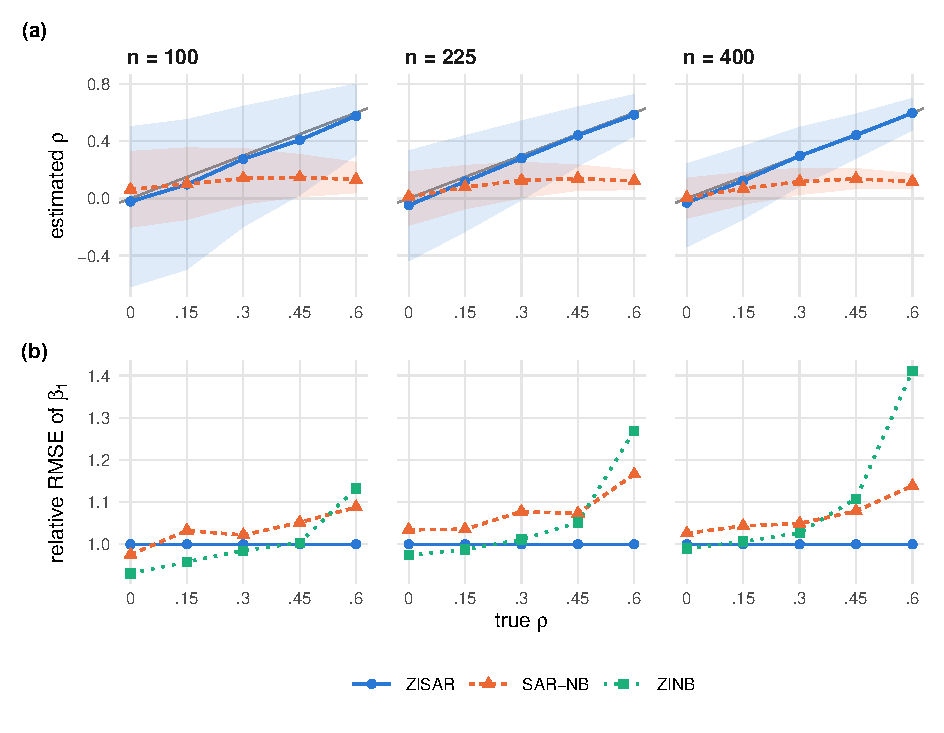
\includegraphics[width=\textwidth]{figures/mc_results.pdf}
\caption{Monte Carlo results, $R = 1{,}000$ replications per scenario. (a) Mean estimate of $\rho$ (lines) and 10th--90th percentiles across replications (bands) for the SAR-NB and ZISAR; the grey line marks the true value. The ZINB fixes $\rho = 0$. (b) RMSE of $\hat\beta_1$ relative to that of ZISAR in the same scenario: values above one favour ZISAR.}\label{fig:mc}
\end{figure}

ZISAR recovers the spatial parameter, whereas the SAR-NB does not (Figure~\ref{fig:mc}a).
Whatever the true value, the SAR-NB estimate stays below 0.15, so that its bias grows with $\rho$ and does not diminish with~$n$: at $\rho=0.6$ it is $-0.47$, $-0.48$ and $-0.48$ for $n = 100$, 225 and 400.
The two-stage procedure ignores the zero-inflated structure and the latent-field formulation, so that its instruments are misspecified.
The mean ZISAR estimate follows the true value at every sample size.
Its bias is small and negative in every scenario, never beyond $-0.052$, and at $\rho=0.6$ and $n=400$ it is $-0.002$, with an RMSE of~$0.087$.
The price is variance when the dependence is weak and the sample is small: at $\rho = 0$ the RMSE of ZISAR is 0.43 with $n=100$ and 0.23 with $n=400$, against 0.25 and 0.12 for the SAR-NB, whose estimate is held near zero.
The RMSE of ZISAR falls with both $n$ and $\rho$, and is below that of the SAR-NB from $\rho = 0.3$ with $n = 400$ and from $\rho = 0.45$ at every sample size.

Ignoring the spatial structure also affects the regression coefficients (Figure~\ref{fig:mc}b).
At $\rho = 0$ the three estimators have similar RMSE; with $n = 100$ ZISAR pays for the two parameters it estimates in vain, $\rho$ and~$\sigma$, with an RMSE of $\hat\beta_1$ 7\% above that of the ZINB, a gap that disappears at $n = 400$.
As $\rho$ grows the ZINB estimator of $\beta_1$ becomes biased upwards, by $0.056$ at $\rho = 0.6$ with $n = 100$ and by $0.066$ with $n = 400$, because the spatially correlated latent field is absorbed into the coefficients; its bias does not shrink with~$n$, whereas that of ZISAR stays below $0.02$ in absolute value in every scenario.
At $\rho = 0.6$ and $n = 400$ the RMSE of $\hat\beta_1$ is $0.079$ for ZISAR, $0.090$ for the SAR-NB and $0.111$ for the ZINB, 14\% and 41\% higher, and the RMSE of $\hat\beta_2$ is $0.072$, $0.084$ and $0.091$.
The efficiency gain of ZISAR grows with $\rho$ and, against the ZINB, with $n$, as the bias of the ZINB becomes the larger part of its RMSE.

The competitors also misattribute the overdispersion.
Because the ZINB estimate of $\kappa$ is occasionally very large, we compare medians.
Both competitors underestimate $\kappa$: the median bias is between $-1.40$ and $-1.52$ for the SAR-NB, which ignores the zero-inflation, and between $-0.70$ and $-1.10$ for the ZINB, growing with $\rho$ as the omitted spatial field adds extra-Poisson variation.
ZISAR has the smallest bias in every scenario, between $-0.34$ and $-0.56$.
The downward bias that remains reflects the trade-off between the random-effects variance $\sigma^2$ and the NB dispersion $\kappa^{-1}$, both of which generate overdispersion, and is accentuated by the exclusion of the fits at the upper bound of~$\kappa$.
ZISAR attains the highest median log-likelihood in every scenario (Table~\ref{tab:mc_kappa}).
Its gap over the ZINB is below one nat at $\rho=0$, where the two models coincide up to the variance component, and grows with $\rho$ and $n$, to 5, 8 and 16 nats at $\rho=0.6$ for $n=100$, $225$ and $400$.
The ZISAR log-likelihood is the Laplace-approximated marginal likelihood, including the Gaussian normalising constant $-\tfrac n2\log(2\pi)$, and the medians are computed over the retained fits, so that the comparison is indicative rather than a formal test, the competitors not being nested in ZISAR in the same way.

Finally, ZISAR converges in 97--100\% of the replications of every scenario.
The fits with $\hat\kappa$ at the upper bound are 12--17\% of the converged ones with $n = 100$, 7--9\% with $n = 225$ and 3--5\% with $n = 400$; keeping them changes the bias and the RMSE of $\hat\beta_1$ and $\hat\beta_2$ by at most $0.005$ and the RMSE of $\hat\rho$ by less than~$0.02$.
A fit, standard errors included, takes on average 0.1\,s with $n=100$, 0.25\,s with $n=225$ and 0.55\,s with $n=400$ on a single core, and the whole experiment, 45{,}000 fits, ran in nine minutes in parallel on a laptop.

% ---------------------------------------------------------------------------
\subsection{Power of tests for spatial dependence}\label{sec:mc_power}

In applied work, the presence of spatial dependence is often judged from Moran's $I$ \citep{moran1950,cliff_ord1973} computed on the residuals of an aspatial model.
In zero-inflated counts this test may lack power, because the spatial signal is diluted by the structural zeros and by negative binomial noise.
We compare it with the likelihood-based tests delivered by ZISAR in a second experiment.
The $n\in\{300, 900\}$ units have centroids drawn uniformly over a $2.5\times2$ box and $\bW$ is the row-standardised 6-nearest-neighbour matrix; four independent standard normal covariates enter the count process and one of them, together with a further independent covariate, enters the inflation process, with
$\bbeta = (1.2,\, 0.4,\, 0.3,\, 0.2,\, -0.15)'$, $\bgamma = (-1.5,\, 0.6,\, -0.4)'$, $\kappa = 2$ and $\sigma = 0.4$.
The covariates are spatially independent, a deliberately unfavourable setting for spatial methods: all the spatial structure in the outcome comes from the latent field.
For each $\rho\in\{0, 0.2, 0.35, 0.5, 0.7\}$ we draw 200 datasets and record how often each test rejects the absence of spatial dependence at the 5\% level (Table~\ref{tab:power_moran}).

\begin{table}[htbp]
\centering
\caption{Rejection rates at the 5\% level of tests for spatial dependence, 200 replications per cell. Zeros range from 35\% ($\rho=0$) to 21\% ($\rho=0.7$).}\label{tab:power_moran}
\small
\begin{tabular}{ll rrrrr}
\toprule
& & \multicolumn{5}{c}{true $\rho$} \\
\cmidrule(lr){3-7}
$n$ & Test & 0 & 0.2 & 0.35 & 0.5 & 0.7 \\
\midrule
\multirow{4}{*}{300}
 & Moran's $I$ on $\by$             & 0.060 & 0.135 & 0.285 & 0.560 & 0.925 \\
 & Moran's $I$ on ZINB residuals    & 0.045 & 0.085 & 0.215 & 0.445 & 0.915 \\
 & ZISAR Wald test on $\tilde\rho$  & 0.035 & 0.240 & 0.492 & 0.840 & 1.000 \\
 & ZISAR LR test of $\rho=0$        & 0.055 & 0.168 & 0.359 & 0.810 & 1.000 \\
\midrule
\multirow{4}{*}{900}
 & Moran's $I$ on $\by$             & 0.065 & 0.170 & 0.490 & 0.875 & 1.000 \\
 & Moran's $I$ on ZINB residuals    & 0.070 & 0.105 & 0.320 & 0.705 & 1.000 \\
 & ZISAR Wald test on $\tilde\rho$  & 0.061 & 0.327 & 0.863 & 1.000 & 1.000 \\
 & ZISAR LR test of $\rho=0$        & 0.086 & 0.276 & 0.817 & 1.000 & 1.000 \\
\bottomrule
\end{tabular}
\end{table}

Under the null all four tests have rejection rates close to the nominal 5\%, with the likelihood-ratio test somewhat liberal at $n=900$ (8.6\%).
Under the alternative the likelihood-based tests are uniformly more powerful.
The gap is largest at moderate dependence: at $\rho=0.35$ the Moran test on ZINB residuals detects the dependence in 22\% of samples with $n=300$ and 32\% with $n=900$, against 49\% and 86\% for the ZISAR Wald test.
The Moran test on residuals is also less powerful than the same test on the raw counts, because the aspatial model partly absorbs the spatial signal into its intercept and dispersion.
In zero-inflated count settings, a non-significant Moran statistic on residuals is therefore weak evidence of spatial independence, and inference on spatial dependence should rest on the structural parameter.


\section{Empirical Application: Domestic Solar PV Adoption in England}\label{sec:solar}

% ---------------------------------------------------------------------------
\subsection{Motivation and data}\label{sec:solar_data}

The diffusion of rooftop solar photovoltaic (PV) systems displays the three features that motivate ZISAR.
First, adoption is spatially contagious: households are more likely to install panels when neighbours have done so, through visibility, word of mouth and local installer activity, as documented for the United States \citep{bollinger_gillingham2012,graziano_gillingham2015,kwan2012}, Germany \citep{rode_weber2016,dharshing2017,schaffer_brun2015} and the United Kingdom \citep{balta_ozkan2015,snape2016}.
Second, small-area counts contain zeros of two different kinds.
In neighbourhoods dominated by purpose-built blocks of flats, no household controls a roof and domestic installation is infeasible: these are \emph{structural} zeros.
In neighbourhoods of houses, a zero over a given period only means that no household happened to adopt: these are \emph{sampling} zeros of a positive-intensity process.
Third, intensities vary widely with income, tenure, housing stock and local markets, producing overdispersion.
The application therefore asks for both parts of the restricted model at once, the spatial parameter and the inflation process, and the direct and indirect effects of Section~\ref{sec:est_effects} are its quantities of interest.

\paragraph{Policy context and outcome.}
The Feed-in Tariff (FiT) scheme, opened in April 2010, paid British households a generation tariff for every kWh produced by small-scale renewable installations.
For domestic PV systems of up to 4\,kW the tariff was 41.3p/kWh at the start, was halved in 2012 and lowered in steps thereafter, and was cut by about two thirds, to 4.39p/kWh, from 8~February 2016; the scheme closed to new applicants in March 2019.
We study the boom that preceded the cut.
In England the scheme accredited about 19{,}000 domestic PV systems of up to 10\,kW in 2010, 158{,}000 in 2011, 125{,}000 in 2012, 75{,}000 in 2013, 103{,}000 in 2014 and 133{,}000 in 2015, against about 20{,}000 a year after the cut.

The window matters for the separation of the two kinds of zeros.
After almost six years of generous tariffs, adoption had reached nearly every neighbourhood where it was feasible: in an area of some 650 households for which the count process predicts tens of installations, a zero is improbable unless installation is infeasible, and the zeros that remain are informative about the housing stock.
After the cut adoption became sparse, and a third of the areas record no installation between 8~February 2016 and March 2019, most of them areas that had adopted before; with intensities of one or two installations per area a zero says little about feasibility, and a spatially dependent count process reproduces clusters of such zeros as sampling zeros.
We therefore model the boom and use the installations after the cut only to validate the structural zeros (Section~\ref{sec:solar_results}).

The outcome is taken from the Ofgem Central FiT Register (installation report of 30~June 2026), which lists every accredited installation with its technology, type, capacity, commissioning date and Lower-layer Super Output Area (LSOA).
We count the domestic PV installations of up to 10\,kW commissioned before 8~February 2016, excluding extensions of existing systems: 611{,}903 installations, of which 4{,}888 were commissioned before April 2010 and joined the scheme when it opened.
The limit of 10\,kW, the upper limit of the second FiT tariff band, keeps the rooftop systems of single houses (typically 2--4\,kW) and leaves out 7{,}089 larger domestic systems (1.1\%).
The register does not geocode 2.4\% of the domestic installations of the window.

The units are the LSOAs of England, small statistical areas of 400--1{,}200 households designed to be socially homogeneous.
The register geocodes installations to the 2001 LSOAs, whereas the 2011 Census and the Indices of Deprivation use the 2011 LSOAs.
For 97\% of the areas the two coincide; where an LSOA was split or merged between the two censuses we aggregate the areas linked by the official best-fit lookup into a single unit, obtaining $n = 32{,}322$ units with a median of 650 households.
The harmonisation matters for a zero-inflated model: matching the register to the 2011 codes directly would assign zero installations to every one of the 1{,}172 LSOAs created in 2011, a spurious excess of zeros.

The number of installations per unit has mean 18.9, variance 396, median 13 and maximum 308; 1{,}112 units (3.4\%) record none and 1{,}323 record one.
Zeros concentrate where the housing stock leaves no roofs to equip: 24\% of the units in the top decile of the share of flats record no installation, against 0.6\% of the units below the median share, and 514 of the 1{,}153 units where flats make up more than 80\% of the household spaces record none.
Greater London has 15\% of the units and 815 of the zeros (73\%): 17\% of its units record no installation, against 1.1\% elsewhere.
The zeros persist after the cut: 873 of the 1{,}112 units without an installation in the boom still had none in March 2019.

\paragraph{Covariates and spatial weights.}
The covariates describe slow-moving characteristics of the areas, measured within the window, and are standardised (Table~\ref{tab:solar_desc}).
The count process includes eleven covariates of its own.
Five are socio-economic: the shares of social-rented households, of residents in managerial and professional occupations (NS-SEC classes 1--2), of residents aged 65 and over and of households with dependent children, from the 2011 Census, and the income-deprivation rate of the English Indices of Deprivation 2019.
Five describe housing and energy: the number of households (log); the share of detached houses; the share of dwellings in Council Tax bands E--H, a measure of property value from the Valuation Office Agency (VOA) stock of properties in 2015; the share of households without gas central heating, who face higher energy costs; and the mean domestic electricity consumption per meter in 2010 (log), from the Department for Energy Security and Net Zero, measured at the start of the scheme because later consumption is net of the panels' self-consumption.
The last is the northing of the population-weighted centroid, which captures the decline of solar irradiation with latitude.

The inflation process includes six variables that can make domestic installation infeasible: the share of household spaces in flats, population density (log) and the shares of private-rented households, of residents in communal establishments such as student halls and care homes, of household spaces with no usual resident and of dwellings built before 1919 (VOA).
These six also enter the count process, since the housing stock shifts the number of eligible roofs even where installation is feasible; their effects on $\E[\by]$ therefore combine the count channel \eqref{eq:effects_count} and the inflation channel \eqref{eq:effects_zero_channel}.

\begin{table}[htbp]
\centering
\caption{Descriptive statistics of the outcome and covariates ($n = 32{,}322$ units). Shares and rates in per cent unless stated; VOA counts are rounded to the nearest ten, so that VOA shares can slightly exceed 100. Sources: Ofgem Central FiT Register; 2011 Census; English Indices of Deprivation 2019; VOA Council Tax stock of properties 2015; DESNZ sub-national electricity consumption 2010.}\label{tab:solar_desc}
\small
\begin{tabular}{lrrrrr}
\toprule
 & Mean & SD & Min & Median & Max \\
\midrule
Domestic PV installations to 7 Feb 2016 & 18.93 & 19.89 & 0 & 13 & 308 \\
\midrule
\multicolumn{6}{l}{\textit{Count process}} \\
\quad Social-rented households & 17.4 & 17.2 & 0.0 & 11.2 & 92.5 \\
\quad Income-deprivation rate & 12.9 & 9.4 & 0.3 & 10.0 & 60.9 \\
\quad Managerial and professional (NS-SEC 1--2) & 31.2 & 12.2 & 2.7 & 30.4 & 78.5 \\
\quad Aged 65 and over & 16.8 & 7.1 & 0.4 & 16.2 & 60.7 \\
\quad Households with dependent children & 29.7 & 7.9 & 2.4 & 29.2 & 72.9 \\
\quad Households (number) & 682.6 & 171.0 & 304 & 650 & 6304 \\
\quad Detached houses & 22.8 & 21.8 & 0.0 & 13.8 & 97.2 \\
\quad Council Tax bands E--H & 18.8 & 23.0 & 0.0 & 8.8 & 102.0 \\
\quad Without gas central heating & 20.3 & 17.9 & 1.6 & 14.6 & 98.7 \\
\quad Electricity per meter, 2010 (kWh) & 4178 & 899 & 1462 & 3982 & 13360 \\
\quad Northing (km) & 276.7 & 127.4 & 10.6 & 260.9 & 654.4 \\
\midrule
\multicolumn{6}{l}{\textit{Inflation and count processes}} \\
\quad Flats (share of household spaces) & 20.0 & 22.2 & 0.0 & 11.6 & 99.7 \\
\quad Population density (per km$^2$) & 4225 & 4154 & 3 & 3430 & 68470 \\
\quad Private-rented households & 16.0 & 11.3 & 1.3 & 12.2 & 87.9 \\
\quad Residents in communal establishments & 1.5 & 4.6 & 0.0 & 0.0 & 86.7 \\
\quad Household spaces with no usual resident & 3.9 & 3.5 & 0.0 & 3.1 & 71.4 \\
\quad Dwellings built before 1919 & 20.8 & 24.3 & 0.0 & 11.3 & 101.4 \\
\bottomrule
\end{tabular}
\end{table}

The spatial weights matrix $\bW$ is the row-standardised queen-contiguity matrix of the generalised (20\,m) LSOA boundaries, with on average 5.86 neighbours per unit; the Isles of Scilly, the only unit without contiguous neighbours, are linked to the nearest unit.
Because $n = 32{,}322$ rules out the dense eigendecomposition, the log-determinant is computed by sparse Cholesky factorisation \eqref{eq:logdet_sparse}.

% ---------------------------------------------------------------------------
\subsection{Estimates}\label{sec:solar_results}

We estimate six specifications.
Three are the benchmarks of the Monte~Carlo study: the negative binomial (NB) regression, the zero-inflated NB (ZINB) and the SAR-NB with the spatial lag $\bW\by$ instrumented by $[\bX,\bW\bX,\bW^2\bX]$.
Three are fitted with the ZISAR template, by the algorithm of Section~\ref{sec:est_algorithm} and the log-determinant \eqref{eq:logdet_sparse}: the restricted ZISAR; the ZINB with Gaussian random effects (ZINB-RE), obtained by fixing $\rho = 0$; and the spatial NB with random effects and no zero-inflation (SAR-NB-RE), obtained by fixing the inflation intercept at $-20$ and its slopes at zero, so that $\pi_i \approx 2\times 10^{-9}$.
The last two are nested in ZISAR, and each removes one of its two parts: the comparison with the ZINB-RE measures what the spatial parameter adds, the comparison with the SAR-NB-RE what the inflation process adds.
A ZISAR fit takes five to six minutes on a laptop (Apple M5 Pro), the effects decomposition under a minute and the bootstrap about two hours on three cores.

\paragraph{Numerical behaviour and inference.}
Started from the default values, the optimiser stops 33 log-likelihood points below the optimum it reaches when started from the SAR-NB-RE estimates, which we report.
At that optimum it stops without declaring convergence, with a largest gradient component of order $10^8$, and the Hessian is not a reliable basis for standard errors.
The cause is the combination of structural zeros with high intensities.
For a unit with no installation whose covariates predict tens, the conditional distribution of $\eta_i$ given $y_i = 0$ has two modes: one near the value implied by the covariates and the neighbours, where the zero is structural, and one far below it, where the zero is a sampling zero of a unit with a very low intensity.
The inner maximisation picks one of them, and where the two have nearly the same height a small change in $\btheta$ makes it switch, so that $\ell_{\mathrm{LA}}$ is not smooth there and the quasi-Newton iterations stall.
A large gradient at the stopping point is also the symptom of the spurious optima that the unit-level field of the general model produces (Appendix~\ref{app:general}), so we check by simulation that this optimum is genuine.
On a data set simulated from the fitted SAR-NB-RE, which has no structural zeros, ZISAR converges without difficulty (largest gradient component 0.7) and estimates 6 structural zeros, with a likelihood-ratio statistic for $\pi_i = 0$ of 0.6.
On a data set simulated from the fitted ZISAR it stops with the same large gradient, but recovers the structural zeros (518 estimated against 511 expected) and the spatial parameter ($\hat\rho = 0.668$ against 0.633), with a likelihood-ratio statistic of 761.
The large gradient thus accompanies structural zeros among units of high intensity, and does not signal a spurious optimum.
For inference we use a parametric bootstrap: $B = 30$ data sets are simulated from the fitted ZISAR and each is refitted from the estimates; the standard errors of the parameters and of the effects are the standard deviations of the replicates.
Only 5 of the 30 replicate fits converge formally, with a median largest gradient component of $7\times 10^7$, yet they show no bias in the quantities of interest: they average $\hat\rho = 0.633$ (range 0.614--0.647) and 511 structural zeros (472--588), the values of the fitted model.
The bootstrap standard errors are close to the Hessian ones for the count process and larger for the inflation process: 0.153 against 0.083 for its intercept and 0.079 against 0.050 for the share of flats.
Because each replicate starts from the estimates, they measure the sampling variability around the reported optimum.
Started from the default values, the fit of the simulated data set above stopped at $\hat\rho = 0.668$, $\hat\sigma = 0.44$ and $\hat\kappa = 20$: the optimiser can stop at different points of the ridge between $\rho$, $\sigma$ and $\kappa$, a source of variation that the bootstrap does not include.

Table~\ref{tab:solar_estimates} reports the estimates of the four main specifications and Table~\ref{tab:solar_fit} the fit of all six.

\begin{table}[htbp]
\centering
\caption{Estimates for domestic PV installations commissioned before 8~February 2016 ($n=32{,}322$ units). Covariates standardised; standard errors in parentheses, from the parametric bootstrap ($B = 30$) for ZISAR. The SAR-NB coefficient on $\widehat{\bW\by}$ (in brackets) multiplies the observed neighbourhood count in the log-mean and is not on the scale of $\rho$. For ZISAR, $\kappa$ is at the upper bound of the optimisation box.}\label{tab:solar_estimates}
\footnotesize
\begin{tabular}{lrrrr}
\toprule
 & NB & ZINB & SAR-NB & ZISAR \\
\midrule
\multicolumn{5}{l}{\textit{Count process} ($\bbeta$)} \\
Intercept                          & $2.693$ (0.004) & $2.712$ (0.004) & $2.128$ (0.015) & $0.895$ (0.016) \\
Social rented                      & $0.216$ (0.010) & $0.226$ (0.010) & $0.135$ (0.010) & $0.019$ (0.006) \\
Income deprivation                 & $0.063$ (0.010) & $0.036$ (0.010) & $0.101$ (0.010) & $0.031$ (0.008) \\
Managerial (NS-SEC 1--2)           & $0.034$ (0.009) & $0.019$ (0.009) & $0.030$ (0.009) & $-0.017$ (0.008) \\
Aged 65 and over                   & $0.006$ (0.008) & $-0.004$ (0.008) & $-0.019$ (0.008) & $-0.019$ (0.005) \\
Dependent children                 & $-0.127$ (0.007) & $-0.117$ (0.008) & $-0.112$ (0.007) & $-0.062$ (0.005) \\
Households (log)                   & $0.201$ (0.005) & $0.194$ (0.005) & $0.171$ (0.005) & $0.146$ (0.004) \\
Detached houses                    & $0.283$ (0.007) & $0.303$ (0.007) & $0.151$ (0.008) & $0.160$ (0.006) \\
Council Tax bands E--H             & $-0.169$ (0.008) & $-0.159$ (0.008) & $-0.074$ (0.008) & $-0.024$ (0.005) \\
Without gas central heating        & $0.029$ (0.007) & $0.057$ (0.007) & $-0.057$ (0.007) & $0.015$ (0.005) \\
Electricity per meter, 2010 (log)  & $-0.012$ (0.008) & $-0.041$ (0.009) & $0.062$ (0.009) & $0.009$ (0.007) \\
Northing                           & $-0.043$ (0.005) & $-0.037$ (0.004) & $-0.007$ (0.005) & $-0.010$ (0.003) \\
Flats                              & $-0.537$ (0.009) & $-0.461$ (0.010) & $-0.381$ (0.010) & $-0.162$ (0.008) \\
Density (log)                      & $-0.173$ (0.007) & $-0.167$ (0.007) & $-0.067$ (0.008) & $-0.056$ (0.005) \\
Private rented                     & $-0.064$ (0.009) & $-0.087$ (0.009) & $-0.081$ (0.009) & $-0.106$ (0.006) \\
Communal establishments            & $0.023$ (0.005) & $0.021$ (0.005) & $0.021$ (0.005) & $0.006$ (0.004) \\
No usual resident                  & $0.048$ (0.005) & $0.046$ (0.005) & $0.012$ (0.005) & $-0.003$ (0.004) \\
Built before 1919                  & $-0.145$ (0.006) & $-0.149$ (0.006) & $-0.116$ (0.006) & $-0.052$ (0.005) \\
$\rho$                             & --- & --- & [$0.028$ (0.001)] & $0.633$ (0.006) \\
\midrule
\multicolumn{5}{l}{\textit{Inflation process} ($\bgamma$)} \\
Intercept                          & --- & $-7.472$ (0.264) & --- & $-6.881$ (0.153) \\
Flats                              & --- & $1.783$ (0.128) & --- & $1.768$ (0.079) \\
Density (log)                      & --- & $1.512$ (0.239) & --- & $0.832$ (0.100) \\
Private rented                     & --- & $-0.238$ (0.075) & --- & $-0.247$ (0.070) \\
Communal establishments            & --- & $0.034$ (0.039) & --- & $0.018$ (0.054) \\
No usual resident                  & --- & $0.010$ (0.075) & --- & $0.097$ (0.059) \\
Built before 1919                  & --- & $-0.518$ (0.092) & --- & $-0.682$ (0.078) \\
\midrule
$\kappa$ (NB shape)                & $2.246$ & $2.363$ & $2.369$ & $500$ \\
$\sigma$ (RE std.\ dev.)           & --- & --- & --- & $0.497$ (0.003) \\
\bottomrule
\end{tabular}
\end{table}

\paragraph{Spatial dependence and structural zeros.}
ZISAR estimates $\hat\rho = 0.633$ (SE 0.006): the latent propensity to adopt of a unit depends strongly on that of its neighbours, and the spatial multiplier $1/(1-\hat\rho) = 2.7$ almost triples the effect of a uniform change in the covariates.
The likelihood-ratio statistic for $\rho = 0$, against the ZINB-RE, is 8{,}463, and the bootstrap $z$ statistic on $\tilde\rho$ is 73.
The spatial lag of the SAR-NB is also significant, and it lowers the AIC of the NB by 1{,}485 points, against 8{,}462 for the latent SAR over the ZINB-RE: an instrumented lag of observed counts captures a small part of the dependence.

The inflation process is driven by housing form.
The probability of a structural zero rises with the share of flats ($\hat\gamma = 1.77$) and with density ($0.83$) and, given these, is lower where the stock was built before 1919 ($-0.68$), which is consistent with old terraced houses, each with a roof of its own, as opposed to purpose-built blocks, and where private renting is more common ($-0.25$); communal establishments and vacant dwellings have no significant role.
The fitted probabilities are very skewed: the median $\hat\pi_i$ is 0.0008 and the 99th percentile 0.45; they average less than 0.003 in each of the first four quintiles of the share of flats and 0.075 in the fifth.
The model expects 511 structural zeros, 46\% of the 1{,}112 observed, and 463 observed zeros have a posterior probability of being structural above one half.
The structural zeros are concentrated in the urban cores: 75\% of them are in Greater London, and 236 of the 245 units with $\hat\pi_i > 0.5$ are there (Figure~\ref{fig:solar_maps}).

The posterior probability that an observed zero is structural, $P(s_i = 1\mid y_i=0) = \hat\pi_i/[\hat\pi_i + (1-\hat\pi_i)\,h(0;\hat\eta_i,\hat\kappa)]$, can be checked against information the model does not use, namely the installations made after the cut.
A unit without suitable roofs should remain without installations once the tariff falls, whereas a sampling zero of the boom may adopt later.
Among the boom zeros, the posterior probability averages 0.46 for the 873 units still without an installation in March 2019 and 0.28 for the 239 that adopted after the cut.
Ranked by the posterior, the third of the zeros with the lowest values made 0.80 installations per unit after the cut, the middle third 0.28 and the top third 0.18, and the share still at zero rises from 68\% to 80\% and 87\%.
As a classifier of the units that remain at zero, the posterior probability has an area under the ROC curve of 0.63.
The check is conservative: after the cut adoption fell by more than four fifths, so that most sampling zeros of the boom also stay at zero.

\begin{figure}[htbp]
\centering
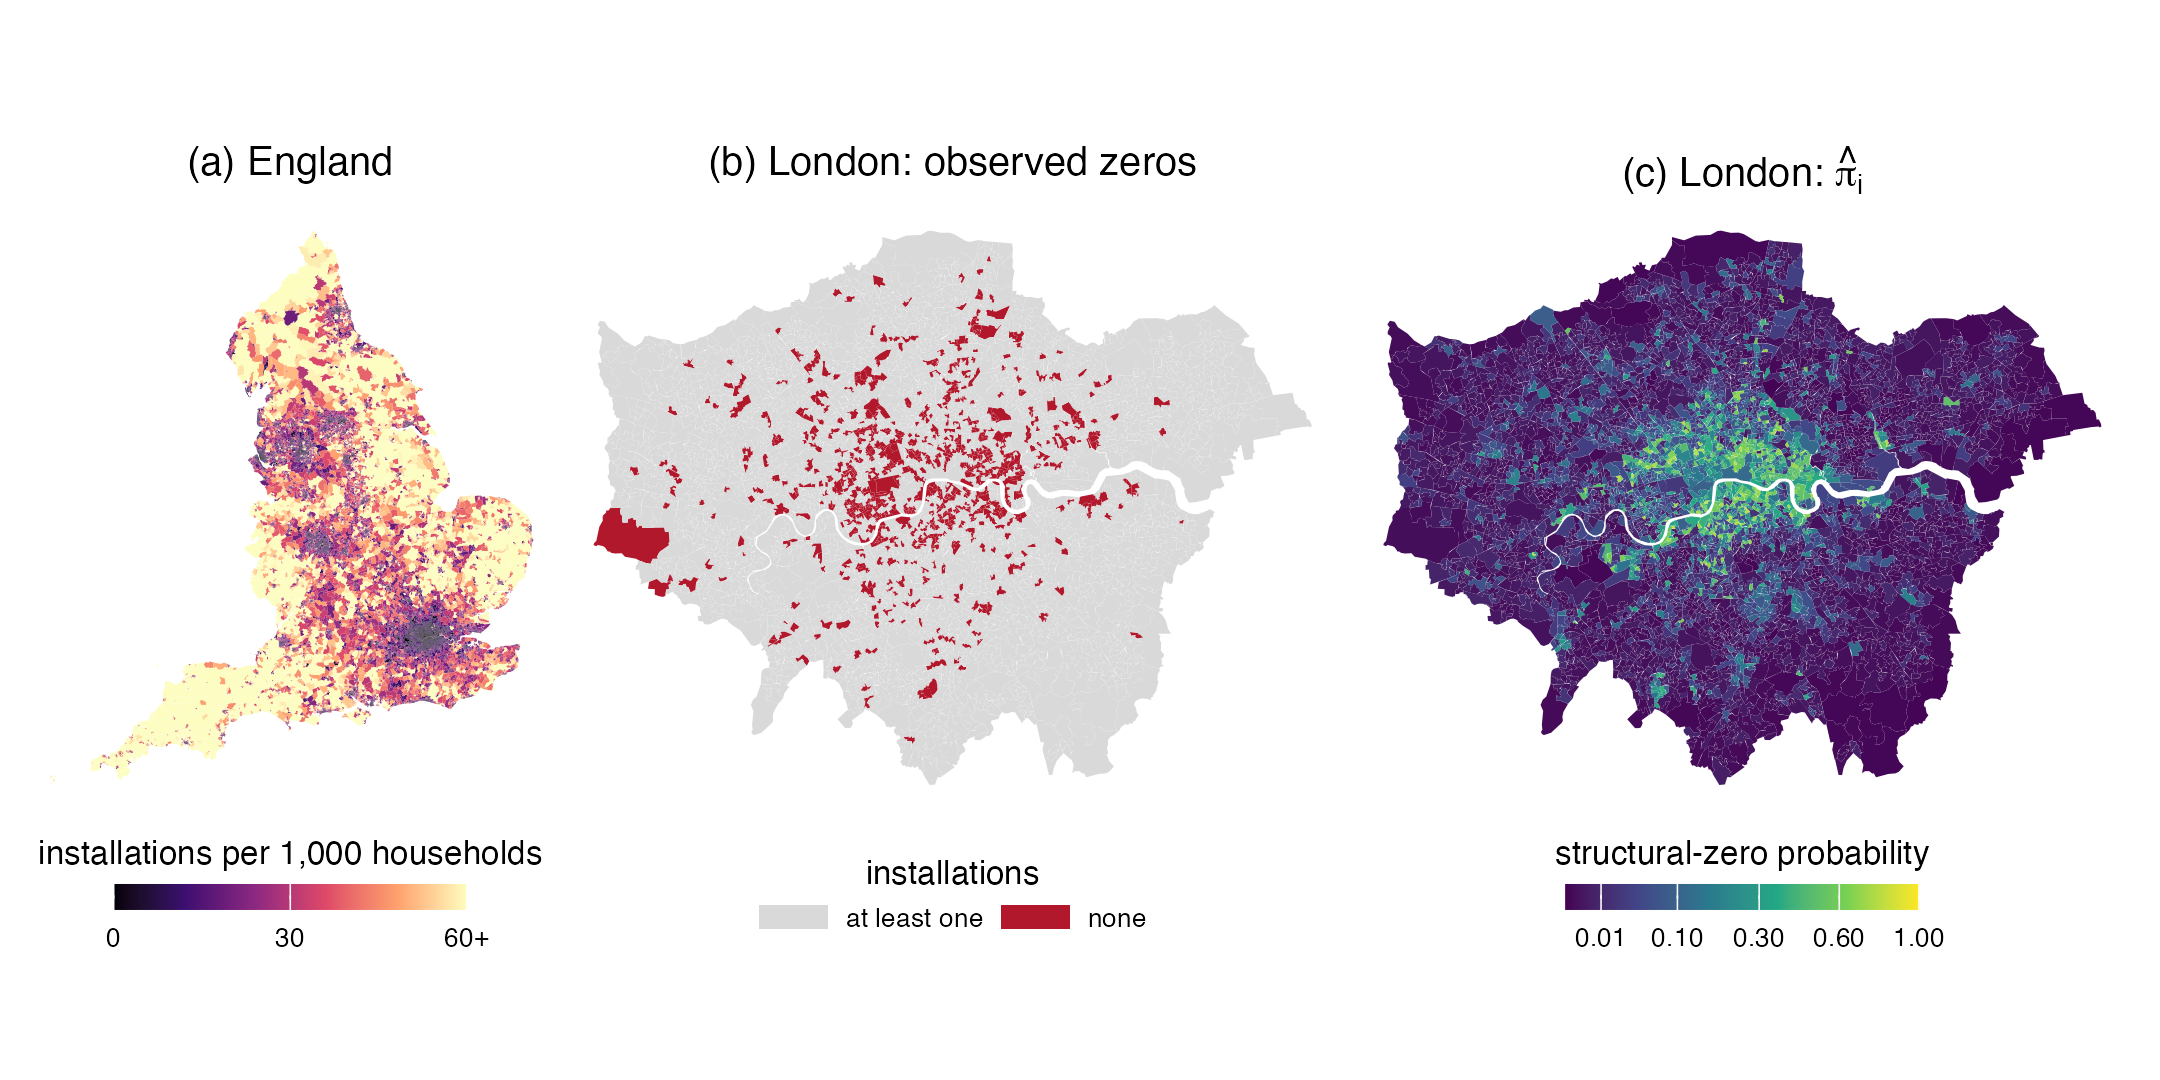
\includegraphics[width=\textwidth]{figures/solar_boom_maps.png}
\caption{(a) Domestic PV installations per 1{,}000 households commissioned before 8~February 2016. (b) London units with no installation in the window. (c) Estimated probability of a structural zero, $\hat\pi_i$, in London: the model assigns a high probability of a structural zero to the inner areas where flats prevail.}\label{fig:solar_maps}
\end{figure}

\paragraph{Covariate effects and dispersion.}
The coefficients of ZISAR are smaller than those of the aspatial models because they act on the latent predictor before the multiplier; the effects of Table~\ref{tab:solar_effects} are the comparable quantities.
More informative is what changes in relative terms.
The share of social-rented households has a large positive coefficient in the NB and the ZINB (0.216 and 0.226) and the share of dwellings in the upper Council Tax bands a large negative one ($-0.169$ and $-0.159$).
The nested models show where the change comes from: both are still large with independent random effects (0.130 and $-0.179$ in the ZINB-RE) and both shrink by an order of magnitude once the field is spatial (0.020 and $-0.024$ in the SAR-NB-RE, 0.019 and $-0.024$ in ZISAR).
Tenure and property value are spatially clustered, and so is adoption: a model without a spatial field reads the common clustering as an effect of the covariates.
In the same way the coefficients of detached houses and of households with dependent children are halved, and those of managerial occupations and of the elderly share turn from positive to negative.
In ZISAR adoption is higher where there are more households and more detached houses, and lower where flats, private renting, density, pre-1919 dwellings and households with dependent children are more common; it declines from south to north, as does the solar resource.
Given the housing stock, it is also somewhat higher where social renting and income deprivation are more common and lower in the upper Council Tax bands and where managerial occupations prevail, a pattern consistent with the programmes through which social landlords fitted panels to many homes at a time during the boom.

The models without a latent field attribute all the extra-Poisson variation to the NB shape ($\hat\kappa \approx 2.3$).
Once the field is spatial, the shape estimate runs to the upper bound of the optimisation box ($\kappa = 500$), in ZISAR as in the SAR-NB-RE, and the count distribution is effectively Poisson conditional on $\boldsymbol\eta$: the overdispersion is accounted for by the log-normal heterogeneity, $\hat\sigma = 0.497$, filtered through the spatial multiplier.
This is the trade-off between $\sigma^2$ and $\kappa^{-1}$ noted in the Monte~Carlo study, resolved here in favour of the Gaussian component.

\paragraph{Fit and residual dependence.}
Both parts of ZISAR are needed (Table~\ref{tab:solar_fit}).
Adding zero-inflation to the NB lowers the AIC by 1{,}051 points, adding random effects to the ZINB by a further 3{,}140, and making the field spatial by 8{,}462.
Zero-inflation remains relevant when the spatial field is present: ZISAR improves on the SAR-NB-RE by 538 AIC points and 479 BIC points (the likelihood-ratio statistic is 552 on seven restrictions, although the restriction $\pi_i = 0$ lies on the boundary of the parameter space and the $\chi^2_7$ reference is only indicative; the simulation above puts the statistic near zero when there are no structural zeros).
ZISAR has the lowest AIC and BIC of the six specifications, and neither nested model comes close to it.
The three models without zero-inflation under-predict the zeros by about a fifth (887--908 expected against 1{,}112 observed), whereas the zero-inflated ones come close or over-predict (1{,}123 for the ZINB-RE, 1{,}211 for ZISAR and 1{,}269 for the ZINB).

\begin{table}[htbp]
\centering
\caption{Fit of the six specifications and expected number of units with no installation (observed: 1{,}112). Expected zeros are marginal: for the random-effects models the latent field is integrated out by simulation from the fitted distribution (200 draws).}\label{tab:solar_fit}
\small
\begin{tabular}{lrrrrr}
\toprule
 & Log-lik. & $k$ & AIC & BIC & Expected zeros \\
\midrule
NB        & $-117{,}246$ & 19 & $234{,}531$ & $234{,}690$ & $902$ \\
ZINB      & $-116{,}714$ & 26 & $233{,}480$ & $233{,}697$ & $1{,}269$ \\
SAR-NB    & $-116{,}503$ & 20 & $233{,}046$ & $233{,}214$ & $887$ \\
ZINB-RE   & $-115{,}143$ & 27 & $230{,}340$ & $230{,}566$ & $1{,}123$ \\
SAR-NB-RE & $-111{,}187$ & 21 & $222{,}416$ & $222{,}592$ & $908$ \\
ZISAR     & $-110{,}911$ & 28 & $221{,}878$ & $222{,}113$ & $1{,}211$ \\
\bottomrule
\end{tabular}
\end{table}

Moran's $I$ of the counts is 0.550 ($z = 164$ under the normal approximation), and the Pearson residuals of the NB, the ZINB and the SAR-NB retain most of it ($I = 0.34$, $z = 101$--$103$): the covariates and the instrumented lag leave the spatial structure of adoption in the residuals.
The predicted innovations of ZISAR, $\hat\bu = (\mathbf{I}_n-\hat\rho\bW)\hat{\boldsymbol\eta} - \bX\hat\bbeta$, keep a small positive autocorrelation ($I = 0.08$): the latent field absorbs most of the dependence.

% ---------------------------------------------------------------------------
\subsection{Effects decomposition}\label{sec:solar_effects}

Because $\hat\rho$ is large, a coefficient of ZISAR does not measure the effect of its covariate: a change in one unit propagates to its neighbours through the latent field and returns.
Table~\ref{tab:solar_effects} reports the average direct, indirect and total effects on the expected number of installations of a one-standard-deviation increase in each covariate, computed as in Section~\ref{sec:est_effects}, with bootstrap standard errors.
For the six covariates that enter both processes the direct effect includes the inflation channel \eqref{eq:effects_zero_channel}, reported separately in the last column.

\begin{table}[htbp]
\centering
\caption{Average direct, indirect and total effects on the expected number of installations per unit (mean 18.9) of a one-standard-deviation increase in each covariate (ZISAR). Bootstrap standard errors ($B = 30$) in parentheses. The last column is the part of the direct effect that runs through the inflation probability.}\label{tab:solar_effects}
\footnotesize
\begin{tabular}{lrrrr}
\toprule
 & Direct & Indirect & Total & Inflation \\
\midrule
Social rented                      & $0.39$ (0.13) & $0.58$ (0.20) & $0.97$ (0.33) & --- \\
Income deprivation                 & $0.64$ (0.17) & $0.94$ (0.24) & $1.59$ (0.41) & --- \\
Managerial (NS-SEC 1--2)           & $-0.36$ (0.16) & $-0.52$ (0.24) & $-0.88$ (0.40) & --- \\
Aged 65 and over                   & $-0.40$ (0.11) & $-0.59$ (0.16) & $-1.00$ (0.27) & --- \\
Dependent children                 & $-1.29$ (0.11) & $-1.88$ (0.16) & $-3.17$ (0.27) & --- \\
Households (log)                   & $3.05$ (0.09) & $4.46$ (0.16) & $7.50$ (0.24) & --- \\
Detached houses                    & $3.33$ (0.13) & $4.87$ (0.22) & $8.19$ (0.34) & --- \\
Council Tax bands E--H             & $-0.51$ (0.12) & $-0.74$ (0.17) & $-1.25$ (0.28) & --- \\
Without gas central heating        & $0.31$ (0.10) & $0.46$ (0.15) & $0.77$ (0.25) & --- \\
Electricity per meter, 2010 (log)  & $0.19$ (0.14) & $0.27$ (0.21) & $0.46$ (0.35) & --- \\
Northing                           & $-0.21$ (0.06) & $-0.31$ (0.09) & $-0.51$ (0.15) & --- \\
\midrule
Flats                              & $-3.49$ (0.17) & $-4.95$ (0.27) & $-8.43$ (0.43) & $-0.102$ (0.004) \\
Density (log)                      & $-1.22$ (0.10) & $-1.72$ (0.14) & $-2.94$ (0.24) & $-0.048$ (0.007) \\
Private rented                     & $-2.21$ (0.12) & $-3.25$ (0.18) & $-5.45$ (0.30) & $0.014$ (0.004) \\
Communal establishments            & $0.13$ (0.08) & $0.19$ (0.11) & $0.32$ (0.19) & $-0.001$ (0.003) \\
No usual resident                  & $-0.07$ (0.09) & $-0.10$ (0.13) & $-0.17$ (0.22) & $-0.006$ (0.003) \\
Built before 1919                  & $-1.04$ (0.10) & $-1.58$ (0.15) & $-2.62$ (0.25) & $0.039$ (0.005) \\
\bottomrule
\end{tabular}
\end{table}

Indirect effects are the larger part: they account for 59\% of the total effect of every covariate that enters only the count process, a share fixed by $\hat\rho$ and by the weighting of the units by their fitted intensity, and for 58--60\% of the total effect of the other six.
A one-standard-deviation increase in the number of households (log) in every unit raises expected installations by 7.5 per unit, two fifths of the mean, of which 3.0 occurs through the unit's own latent propensity and 4.5 through the feedback from its neighbours; for the share of detached houses the total is 8.2, of which 3.3 is direct.
The share of flats has the largest negative effect ($-8.4$), followed by private renting ($-5.5$), households with dependent children ($-3.2$), density ($-2.9$) and pre-1919 dwellings ($-2.6$).
The inflation channel is small on average, because structural zeros are rare outside the urban cores; it is largest for the share of flats, $-0.10$ out of a direct effect of $-3.49$.
All total effects are distinguishable from zero at the 5\% level except those of electricity consumption, communal establishments and vacant dwellings.
A model with $\rho = 0$ has no indirect effects: the ZINB-RE would report the direct column alone, and the aspatial models a single coefficient per covariate, with the effects of social renting and property value an order of magnitude larger.

The estimate of $\rho$ measures how strongly the latent adoption propensities of neighbouring areas move together, given the covariates.
Peer effects of the kind documented by \citet{bollinger_gillingham2012} and \citet{graziano_gillingham2015} generate such dependence, but so do spatially correlated unobservables---the reach of local installers, roof orientation and shading, local campaigns---and a cross-section cannot separate the two \citep{manski1993,gibbons_overman2012}.
What the application establishes is narrower and, for inference on the covariates, sufficient: treating adoption as spatially independent, or ignoring the structural zeros, distorts the estimated role of tenure, property value, household composition and housing form, leaves strong dependence in the residuals and hides the larger part of every effect.

The restricted model suffices here: the structural zeros follow the housing stock, which the covariates of the inflation process measure.
A spatial field in the inflation predictor would be needed only if the structural zeros clustered beyond what these covariates explain; Appendix~\ref{app:general} shows how such a field can be estimated.



\section{Conclusion}\label{sec:conclusion}

This paper introduced the ZISAR (Zero-Inflated Spatial Autoregressive) model, a unified specification for count data that simultaneously addresses spatial spillovers, zero-inflation, overdispersion, and unobserved unit-level heterogeneity.
The key innovation is the placement of a simultaneous autoregressive structure on the latent linear predictor of the count process---$\boldsymbol{\eta} = (\mathbf{I} - \rho\bW)^{-1}(\bX\bbeta + \bu)$---rather than on the observed count.
This SAR-on-$\boldsymbol{\eta}$ formulation preserves the direct/indirect/total effects decomposition that is central to the spatial econometrics programme \citep{lesage_pace2009,arbia2006} while avoiding the endogeneity of observed spatial lags that complicates SAR-on-$\by$ specifications \citep{lambert2010}.
Simultaneously, it differs from CAR-based spatial random-effects models \citep{lee2013,neelon2013} by providing a structural, single-parameter characterisation of spatial dependence with an explicit spillover interpretation.

Estimation by Laplace-approximated marginal likelihood, implemented via \texttt{TMB} \citep{kristensen2016}, yields a computationally efficient and scalable algorithm.
The sparse-matrix operations and automatic differentiation exploited by \texttt{TMB} echo the computational concerns raised by \citet{arbia_nardelli2024} and \citet{arbia_nardelli_salvini} in the context of pairwise pseudo-likelihood for large spatial datasets.
We established consistency and asymptotic normality of the estimator and derived the effects decomposition for the nonlinear zero-inflated mixture.

The Monte~Carlo study confirmed that ignoring either spatial dependence or zero-inflation leads to substantial bias: the standard ZINB inflates covariate effects when $\rho > 0$, while the SAR-NB severely underestimates the spatial lag when structural zeros are present, with a bias that does not vanish as $n$ grows.
ZISAR recovers the data-generating parameters with low bias and an RMSE that decreases with $n$.
A second experiment showed that residual-based Moran tests can miss spatial dependence that the likelihood detects.

The application took the estimator to the $n = 32{,}322$ small areas of England, where a fit takes five to six minutes on a laptop.
On domestic solar PV installations during the boom of the Feed-in Tariff, before the tariff cut of 2016, it needs both parts of the restricted model.
Adoption is strongly dependent in space ($\hat\rho = 0.63$, likelihood ratio 8{,}463 against the ZINB with random effects), and zero-inflation remains needed once the spatial field is in (likelihood ratio 552 against the SAR-NB-RE), so that ZISAR has the lowest AIC and BIC of six specifications.
The structural zeros follow the housing stock: nearly half of the observed zeros are structural, three quarters of them are in Greater London, and their posterior probabilities are higher where areas remained without installations after the cut, which the model does not use.
The aspatial models read the common clustering of tenure, property value and adoption as effects of the covariates, which shrink by an order of magnitude in ZISAR, and they have no counterpart to the indirect effects, which are about 60\% of every total effect.
The window is chosen so that zeros are informative: during the boom so many installations are expected in most areas that a zero is improbable under the count process, whereas after the cut, with one or two installations per area, a spatially dependent count process reproduces clusters of zeros as sampling zeros.
The same high intensities make the Laplace objective non-smooth, and the optimiser stops with a large gradient at an optimum that a simulation from the fitted model shows to be genuine; a parametric bootstrap provides the standard errors.

The general model, with a spatial field in the inflation predictor, is not needed in this application, since the covariates explain where the structural zeros are.
Where it is, the simulations of Appendix~\ref{app:general} show that it should be estimated with a reduced-rank field on a lattice of knots, which the Laplace approximation handles, rather than with a field of one element per unit, which produces likelihood-ratio statistics in the thousands on data that contain no field at all.

\paragraph{Limitations.}
Four limitations warrant acknowledgement.
First, the Laplace approximation may lose accuracy when the conditional posterior of $\boldsymbol{\eta}$ is highly non-Gaussian (e.g.\ for very sparse data with many zero counts); higher-order Laplace corrections or adaptive quadrature could improve precision in such settings.
With the unit-level field of the general model it produced spurious optima, with gradients of order $10^8$ at the stopping point and log-likelihoods thousands of points above their true value (Appendix~\ref{app:general}).
A large gradient at the stopping point flags them but is not specific: with structural zeros among units of high intensity, as in the solar application, the conditional posterior of $\eta_i$ of a zero unit has two modes and the optimiser stops with a large gradient at a genuine optimum, so that a simulation from the fitted model is needed to tell the two cases apart, and a parametric bootstrap replaces the Hessian standard errors.
Second, the unit-level random effects $\bu$ are assumed independent Gaussian; correlated or non-Gaussian specifications would add flexibility at the cost of a more complex \texttt{TMB} template.
Third, the eigenvalue pre-computation for the log-determinant $\log|\det(\mathbf{I}-\rho\bW)|$ is $O(n^3)$; the sparse-Cholesky alternative of \eqref{eq:logdet_sparse} removes this bottleneck at the national scale of the application, but its cost grows with the fill-in of the Cholesky factor, so that for dense weights matrices or $n$ in the millions stochastic log-determinant approximations \citep[e.g.][]{barry_pace1999} would be needed.
Fourth, the general specification with a unit-level field in the inflation predictor is poorly served by the Laplace approximation: each element of the field is informed by a single outcome that is zero or not, the approximation error accumulates over the units, and on data generated without a field the approximate likelihood-ratio statistic runs into the thousands.
The reduced-rank field on a lattice of knots removes the failure and is estimated without difficulty on simulated data at the national scale, at the price of a resolution set by the knot spacing: a field whose variance lies below the spacing is detected but not reconstructed (Appendix~\ref{app:general}), and as the spacing falls towards the size of the units the unit-level case and its failure return.
Simulation-based inference on the same \texttt{TMB} template, such as Hamiltonian Monte Carlo, remains the route to a unit-level field.

\paragraph{Extensions.}
Several directions for future research emerge naturally.
The most immediate is the incorporation of \emph{temporal dependence}, yielding a spatio-temporal ZISAR of the form
\[
  \eta_{it} = \rho(\bW\boldsymbol{\eta}_t)_i + \phi\,\eta_{i,t-1} + \mathbf{x}_{it}'\bbeta + u_i + \nu_t,
\]
where $\phi$ captures persistence and $\nu_t$ is a time-specific effect.
The panel structure introduces additional identification and computational challenges (dynamic spatial panel asymptotics, high-dimensional latent field) that merit a dedicated treatment.

A second extension concerns alternative spatial structures: replacing the single $\bW$ with multiple weight matrices (e.g.\ geographic and economic proximity), or letting $\bW$ be endogenous.

Third, the ZISAR template naturally accommodates other count distributions (generalised Poisson, Conway--Maxwell--Poisson) and alternative inflation links (probit, complementary log-log) by modifying the observation-model block of the \texttt{TMB} template.

Finally, automated tools for choosing among the restricted and general specifications, and among weights matrices, would make the \texttt{zisar} package \citep{zisar_pkg} easier to use in applied work.


\newpage
\bibliography{references}

\newpage
\appendix
\section{Proofs}\label{app:proofs}

% ---------------------------------------------------------------------------
\subsection{Proof of Proposition~\ref{prop:consistency}}\label{app:proof_consistency}

We verify the conditions of the extremum-estimator consistency theorem \citep[Theorem~2.1]{newey_mcfadden1994}.

\paragraph{Laplace approximation error.}
Let $\ell(\btheta) = \log\int p(\by,\boldsymbol{\eta}\mid\btheta)\,\mathrm{d}\boldsymbol{\eta}$ denote the exact marginal log-likelihood and $\ell_{\mathrm{LA}}(\btheta)$ the Laplace approximation \eqref{eq:laplace}.
By \citet{tierney_kadane1986}, $|\ell_{\mathrm{LA}}(\btheta) - \ell(\btheta)| = O(1)$ uniformly over $\Theta$ (the error is bounded because the conditional density $f(y_i\mid\eta_i,\pi_i;\,\kappa)$ has bounded derivatives in $\eta_i$ under Assumption~\ref{ass:param}).
Dividing by $n$: $|n^{-1}\ell_{\mathrm{LA}}(\btheta) - n^{-1}\ell(\btheta)| = O(n^{-1}) \to 0$.

\paragraph{Uniform convergence.}
The exact marginal log-likelihood satisfies $n^{-1}\ell(\btheta) \to Q(\btheta) \equiv \E[\log p(y_1\mid\btheta)]$ uniformly over $\Theta$, by the uniform law of large numbers.
The key requirement is that the summands are bounded and equicontinuous in $\btheta$, which holds under the compactness of $\Theta$ (Assumption~\ref{ass:param}) and the boundedness of $\bW$ (Assumption~\ref{ass:W}).
Combined with the vanishing Laplace error, $\sup_{\btheta\in\Theta}|n^{-1}\ell_{\mathrm{LA}}(\btheta) - Q(\btheta)| \plim 0$.

\paragraph{Identification.}
By Assumption~\ref{ass:identification}, $Q(\btheta)$ has a unique maximum at $\btheta_0$.

Finally, compactness of $\Theta$, uniform convergence, and identifiable uniqueness satisfy the conditions of the extremum-estimator theorem, giving $\hat{\btheta}_n \plim \btheta_0$.
\hfill$\square$

% ---------------------------------------------------------------------------
\subsection{Proof of Proposition~\ref{prop:normality}}\label{app:proof_normality}

\paragraph{Score expansion.}
By a mean-value expansion around $\btheta_0$:
\[
  \mathbf{0} = n^{-1/2}\frac{\partial\ell_{\mathrm{LA}}}{\partial\btheta}\bigg|_{\hat{\btheta}}
  = n^{-1/2}\frac{\partial\ell_{\mathrm{LA}}}{\partial\btheta}\bigg|_{\btheta_0}
  + n^{-1}\frac{\partial^2\ell_{\mathrm{LA}}}{\partial\btheta\,\partial\btheta'}\bigg|_{\bar{\btheta}}\;
  \sqrt{n}(\hat{\btheta} - \btheta_0).
\]

\paragraph{CLT for the score.}
The Laplace-approximate score $\partial\ell_{\mathrm{LA}}/\partial\btheta$ can be decomposed as a sum of local contributions $s_i(\btheta)$ that depend on unit $i$ and its spatial neighbours.
Under Assumption~\ref{ass:W}, the spatial weights have uniformly bounded row and column sums, so each $s_i$ depends on at most $O(1)$ other units (the neighbourhood is bounded).
This induces a mixing structure that satisfies the CLT for spatially dependent arrays \citep[see][Theorem~3.1]{lee2004}:
\[
  n^{-1/2}\sum_{i=1}^n s_i(\btheta_0) \dlim N\!\bigl(\mathbf{0},\,\boldsymbol{\Omega}_0\bigr),
\]
where $\boldsymbol{\Omega}_0 = \lim_{n\to\infty} \Var\bigl[n^{-1/2}\sum_i s_i(\btheta_0)\bigr]$.

\paragraph{Hessian convergence.}
By the uniform LLN,
\[
  n^{-1}\frac{\partial^2\ell_{\mathrm{LA}}}{\partial\btheta\,\partial\btheta'}\bigg|_{\bar{\btheta}}
  \plim \mathcal{H}_0 \equiv \E\!\left[\frac{\partial^2 \log p(y_1\mid\btheta)}{\partial\btheta\,\partial\btheta'}\bigg|_{\btheta_0}\right],
\]
which is negative definite by Assumption~\ref{ass:identification}.
Under standard regularity (information matrix equality), $\mathcal{H}_0 = -\mathcal{I}(\btheta_0) = -\boldsymbol{\Omega}_0$.

Combining these results and rearranging the score expansion,
\[
  \sqrt{n}(\hat{\btheta} - \btheta_0) = -\mathcal{H}_0^{-1}\;n^{-1/2}\sum_i s_i(\btheta_0) + o_p(1) \dlim N\!\bigl(\mathbf{0},\,\mathcal{I}(\btheta_0)^{-1}\bigr).
\]
\hfill$\square$

% ---------------------------------------------------------------------------
\subsection{Proof of Proposition~\ref{prop:effects}}\label{app:proof_effects}

Under the restricted ZISAR ($\mathbf{g}=\mathbf{0}$), the marginal expectation of $y_i$ evaluated at the conditional mode is
\[
  \E[y_i] \approx (1 - \pi_i)\,\mu_i, \qquad \mu_i = \exp(\eta_i), \quad \pi_i = \logit^{-1}(\mathbf{z}_i'\bgamma).
\]

The latent predictor at the mode satisfies $\hat{\boldsymbol{\eta}} \approx \mathbf{S}(\rho)\bX\bbeta$ (ignoring the random-effect contribution, which integrates out at the mode).
The partial derivative of $\boldsymbol{\eta}$ with respect to $x_{jr}$ is
\[
  \frac{\partial\eta_i}{\partial x_{jr}} = [\mathbf{S}(\rho)]_{ij}\,\beta_r.
\]
The effect on $\E[y_i]$ is
\[
  \frac{\partial\E[y_i]}{\partial x_{jr}} = (1-\pi_i)\,\mu_i\,[\mathbf{S}(\rho)]_{ij}\,\beta_r + \underbrace{(\text{inflation channel})}_{\text{diagonal only}}.
\]
Stacking: $\mathbf{M}_r = \diag((1-\hat{\bpi})\odot\hat{\bmu})\,\mathbf{S}(\rho)\,\beta_r$.

\textbf{(i)} When $\rho \in [0,1)$ and $\bW \geq 0$ entrywise, the power-series $\mathbf{S}(\rho) = \sum_{s=0}^\infty \rho^s\bW^s$ has all non-negative entries.
Since $(1-\pi_i)\mu_i > 0$, $\mathbf{M}_r$ has the same sign as $\beta_r$.

\textbf{(ii)} When $\rho = 0$, $\mathbf{S}(\rho) = \mathbf{I}_n$ and $\mathbf{M}_r$ is diagonal, so all indirect effects (off-diagonal elements) are zero.
For $\rho \neq 0$, $\mathbf{S}(\rho)$ has positive off-diagonal elements (since $\bW^s$ has positive entries for $s \geq 1$ on connected lattices), making indirect effects non-zero.

\textbf{(iii)} Each element of $\mathbf{S}(\rho) = \sum_{s=0}^\infty \rho^s\bW^s$ is monotonically increasing in $|\rho|$ for $\rho \geq 0$ (since all terms $\rho^s[\bW^s]_{ij}$ are non-negative and increasing in $\rho$).
\hfill$\square$

% =============================================================================
\section{Monte Carlo Tables}\label{app:mc}

Tables~\ref{tab:mc_beta}--\ref{tab:mc_kappa} report the results of the experiment of Section~\ref{sec:montecarlo} for three of the five values of~$\rho$; the summaries for all fifteen scenarios are produced by \texttt{mc\_figure.r}.

\begin{table}[htbp]
\centering
\caption{Monte Carlo bias and RMSE of $\hat{\beta}_1$ ($\beta_1^0 = 0.8$) and $\hat{\beta}_2$ ($\beta_2^0 = -0.5$), $R=1{,}000$ replications per scenario. The ZISAR summaries exclude the fits with $\hat\kappa > 100$ and use 810--963 fits per scenario.}\label{tab:mc_beta}
\footnotesize
\setlength{\tabcolsep}{4pt}
\begin{tabular}{ll rrr rrr rrr}
\toprule
& & \multicolumn{3}{c}{$\rho=0$} & \multicolumn{3}{c}{$\rho=0.3$} & \multicolumn{3}{c}{$\rho=0.6$} \\
\cmidrule(lr){3-5}\cmidrule(lr){6-8}\cmidrule(lr){9-11}
& Model & $n{=}100$ & $n{=}225$ & $n{=}400$ & $n{=}100$ & $n{=}225$ & $n{=}400$ & $n{=}100$ & $n{=}225$ & $n{=}400$ \\
\midrule
\multicolumn{11}{l}{\emph{Panel A: $\hat{\beta}_1$}} \\[3pt]
\multirow{3}{*}{Bias}
  & ZISAR    & $-0.019$ & $-0.005$ & $-0.001$ & $-0.013$ & $0.002$ & $0.000$ & $-0.007$ & $-0.004$ & $0.001$ \\
  & SAR-NB   & $-0.009$ & $-0.004$ & $-0.002$ & $-0.010$ & $-0.000$ & $-0.000$ & $-0.004$ & $-0.003$ & $0.002$ \\
  & ZINB     & $0.001$ & $0.001$ & $0.004$ & $0.008$ & $0.019$ & $0.015$ & $0.056$ & $0.057$ & $0.066$ \\
[3pt]
\multirow{3}{*}{RMSE}
  & ZISAR    & $0.188$ & $0.110$ & $0.083$ & $0.173$ & $0.112$ & $0.080$ & $0.163$ & $0.101$ & $0.079$ \\
  & SAR-NB   & $0.184$ & $0.113$ & $0.086$ & $0.177$ & $0.120$ & $0.084$ & $0.177$ & $0.117$ & $0.090$ \\
  & ZINB     & $0.175$ & $0.107$ & $0.083$ & $0.170$ & $0.113$ & $0.082$ & $0.185$ & $0.128$ & $0.111$ \\
\midrule
\multicolumn{11}{l}{\emph{Panel B: $\hat{\beta}_2$}} \\[3pt]
\multirow{3}{*}{Bias}
  & ZISAR    & $0.008$ & $0.000$ & $0.000$ & $0.003$ & $0.008$ & $0.005$ & $0.003$ & $-0.003$ & $0.001$ \\
  & SAR-NB   & $0.002$ & $-0.003$ & $0.001$ & $0.004$ & $0.010$ & $0.004$ & $0.005$ & $-0.001$ & $0.001$ \\
  & ZINB     & $-0.003$ & $-0.006$ & $-0.002$ & $-0.007$ & $-0.001$ & $-0.006$ & $-0.033$ & $-0.040$ & $-0.041$ \\
[3pt]
\multirow{3}{*}{RMSE}
  & ZISAR    & $0.168$ & $0.108$ & $0.078$ & $0.159$ & $0.105$ & $0.073$ & $0.152$ & $0.091$ & $0.072$ \\
  & SAR-NB   & $0.176$ & $0.110$ & $0.080$ & $0.168$ & $0.111$ & $0.080$ & $0.176$ & $0.107$ & $0.084$ \\
  & ZINB     & $0.165$ & $0.107$ & $0.079$ & $0.161$ & $0.104$ & $0.075$ & $0.176$ & $0.116$ & $0.091$ \\
\bottomrule
\end{tabular}
\end{table}

\begin{table}[htbp]
\centering
\caption{Monte Carlo bias and RMSE of $\hat{\rho}$, $R=1{,}000$ replications per scenario. The ZINB does not estimate~$\rho$.}\label{tab:mc_rho}
\footnotesize
\setlength{\tabcolsep}{4pt}
\begin{tabular}{ll rrr rrr rrr}
\toprule
& & \multicolumn{3}{c}{$\rho=0$} & \multicolumn{3}{c}{$\rho=0.3$} & \multicolumn{3}{c}{$\rho=0.6$} \\
\cmidrule(lr){3-5}\cmidrule(lr){6-8}\cmidrule(lr){9-11}
& Model & $n{=}100$ & $n{=}225$ & $n{=}400$ & $n{=}100$ & $n{=}225$ & $n{=}400$ & $n{=}100$ & $n{=}225$ & $n{=}400$ \\
\midrule
\multirow{2}{*}{Bias}
  & SAR-NB   & $0.063$ & $0.011$ & $0.005$ & $-0.160$ & $-0.174$ & $-0.182$ & $-0.467$ & $-0.477$ & $-0.482$ \\
  & ZISAR    & $-0.022$ & $-0.048$ & $-0.029$ & $-0.024$ & $-0.019$ & $-0.002$ & $-0.021$ & $-0.013$ & $-0.002$ \\
[3pt]
\multirow{2}{*}{RMSE}
  & SAR-NB   & $0.253$ & $0.161$ & $0.115$ & $0.244$ & $0.204$ & $0.196$ & $0.477$ & $0.480$ & $0.484$ \\
  & ZISAR    & $0.433$ & $0.311$ & $0.227$ & $0.338$ & $0.228$ & $0.161$ & $0.229$ & $0.127$ & $0.087$ \\
\bottomrule
\end{tabular}
\end{table}

\begin{table}[htbp]
\centering
\caption{Monte Carlo median bias of $\hat{\kappa}$ ($\kappa^0=2$) and median log-likelihood, $R=1{,}000$ replications per scenario.}\label{tab:mc_kappa}
\footnotesize
\setlength{\tabcolsep}{4pt}
\begin{tabular}{ll rrr rrr rrr}
\toprule
& & \multicolumn{3}{c}{$\rho=0$} & \multicolumn{3}{c}{$\rho=0.3$} & \multicolumn{3}{c}{$\rho=0.6$} \\
\cmidrule(lr){3-5}\cmidrule(lr){6-8}\cmidrule(lr){9-11}
& Model & $n{=}100$ & $n{=}225$ & $n{=}400$ & $n{=}100$ & $n{=}225$ & $n{=}400$ & $n{=}100$ & $n{=}225$ & $n{=}400$ \\
\midrule
\multicolumn{11}{l}{\emph{Panel A: Median bias of $\hat{\kappa}$}} \\[3pt]
  & ZISAR    & $-0.452$ & $-0.511$ & $-0.565$ & $-0.403$ & $-0.523$ & $-0.496$ & $-0.422$ & $-0.353$ & $-0.340$ \\
  & SAR-NB   & $-1.402$ & $-1.428$ & $-1.438$ & $-1.418$ & $-1.448$ & $-1.460$ & $-1.493$ & $-1.511$ & $-1.517$ \\
  & ZINB     & $-0.700$ & $-0.787$ & $-0.860$ & $-0.714$ & $-0.870$ & $-0.896$ & $-0.980$ & $-1.069$ & $-1.103$ \\
\midrule
\multicolumn{11}{l}{\emph{Panel B: Median log-likelihood}} \\[3pt]
  & ZISAR    & $-159$ & $-364$ & $-649$ & $-175$ & $-397$ & $-711$ & $-214$ & $-491$ & $-872$ \\
  & SAR-NB   & $-162$ & $-369$ & $-656$ & $-178$ & $-403$ & $-719$ & $-221$ & $-500$ & $-889$ \\
  & ZINB     & $-160$ & $-365$ & $-650$ & $-176$ & $-399$ & $-713$ & $-220$ & $-499$ & $-887$ \\
\bottomrule
\end{tabular}
\end{table}

\clearpage

\section{Spatial Inflation Predictor: Simulation Checks}\label{app:general}

To assess the Laplace-approximate estimator of the general ZISAR (Section~\ref{sec:model_spec}), we simulate from it on regular lattices with row-standardised queen contiguity, 24 replications for each of $n = 900$, 3600 and 10{,}000, with two i.i.d.\ $N(0,1)$ count covariates, one inflation covariate, $\bbeta = (1,\, 0.5,\, -0.3)'$, $\rho = 0.4$, $\sigma = 0.5$, $\kappa = 2$, $\bgamma = (-1,\, 0.8)'$, $\rho_0 = 0.6$ and $\sigma_0 = 1$.
About 40\% of the simulated counts are zero, four fifths of them structural.
All 72 fits converge, none has a positive Laplace log-likelihood, and the largest gradient component at the optimum is below 0.1.

\begin{table}[htbp]
\centering
\caption{General ZISAR estimated by Laplace approximation on simulated lattices: mean (standard deviation) over 24 replications.}\label{tab:general_mc}
\small
\begin{tabular}{lcccc}
\toprule
 & True & $n = 900$ & $n = 3600$ & $n = 10{,}000$ \\
\midrule
$\beta_1$   & $0.5$  & $0.508$ (0.040) & $0.496$ (0.017) & $0.498$ (0.014) \\
$\beta_2$   & $-0.3$ & $-0.289$ (0.043) & $-0.288$ (0.021) & $-0.304$ (0.012) \\
$\rho$      & $0.4$  & $0.406$ (0.094) & $0.428$ (0.064) & $0.416$ (0.035) \\
$\sigma$    & $0.5$  & $0.443$ (0.111) & $0.441$ (0.041) & $0.444$ (0.027) \\
$\gamma_0$  & $-1$   & $-0.853$ (0.121) & $-0.853$ (0.082) & $-0.867$ (0.038) \\
$\gamma_1$  & $0.8$  & $0.669$ (0.091) & $0.693$ (0.060) & $0.693$ (0.030) \\
$\rho_0$    & $0.6$  & $0.748$ (0.377) & $0.853$ (0.056) & $0.870$ (0.030) \\
$\sigma_0$  & $1$    & $0.344$ (0.089) & $0.295$ (0.065) & $0.288$ (0.040) \\
\bottomrule
\end{tabular}
\end{table}

Table~\ref{tab:general_mc} shows that the count process is recovered as well as under the restricted model: $\bbeta$ and $\rho$ are close to their true values, and $\sigma$ is slightly underestimated, the trade-off with $\kappa$ noted in Section~\ref{sec:montecarlo}.
The inflation process is not.
At every sample size $\sigma_0$ is estimated at about 0.3 instead of 1 and $\rho_0$ at 0.75--0.87 instead of 0.6, and the inflation coefficients are attenuated by 13--17\%.
The bias does not shrink with $n$, because the number of random effects grows with the data and each $g_i$ is informed by a single observation that is zero or not, the setting in which the Laplace approximation of binary-response random effects is known to be most biased \citep{joe2008}.
The approximation replaces a rough field with a smoother one of much smaller variance.
With this estimator $\sigma_0$, $\rho_0$ and, to a lesser extent, $\bgamma$ should not be read at face value, and at the national scale the failure is worse, as the next check shows; the reduced-rank field of Section~\ref{sec:model_spec} is the alternative adopted in the paper.

\paragraph{Reduced-rank field at the national scale.}
The second check uses a design at the scale of the application, built on an outcome with many structural zeros: shoplifting, which cannot be recorded where there are no shops.
The units and the weights matrix are the 32{,}322 units of Section~\ref{sec:solar_data}.
The count process has six covariates---retail and non-retail employment at the workplace (Business Register and Employment Survey 2018, log of one plus), residents (log), population density (log), the income-deprivation rate and the social-rented share---and the inflation process three: an indicator of no recorded retail employment, retail employment and density.
The parameters are the restricted ZISAR estimates for the shoplifting offences recorded by the police in each unit between July 2016 and June 2019 (\texttt{data.police.uk}; 33.9\% of the units record none), which give $\hat\rho = 0$ and attribute 45\% of the zeros to the structural regime.
From these four datasets are simulated with different fields in the inflation predictor: no field; a field of the reduced-rank form \eqref{eq:rr_g} on knots 10~km apart, with $\rho_0 = 0.9$ and $\sigma_0 = 0.5$; a field constant within the areas of the 38 police forces, drawn from $N(0, 0.7^2)$ for each force, the step field that differences of recording between forces would produce; and the unit-level SAR field of the general model, with $\rho_0 = 0.9$ and $\sigma_0 = 0.5$.
Each dataset receives a restricted fit and then the reduced-rank field on the lattice of knots 10~km apart ($K = 1{,}499$ knots, bisquare radius 15~km, about seven knots per unit), by the profile procedure of Appendix~\ref{app:tmb} (\texttt{crime\_application.r}); Table~\ref{tab:general_sim} reports the results.

\begin{table}[htbp]
\centering
\caption{Reduced-rank inflation field (10~km knots) on data simulated at the national scale: likelihood-ratio statistic against the restricted fit, field estimates and correlation between the predicted and the true field. The last row fits the unit-level field of the general model to the data without a field. Bounds of the optimisation box: $\rho_0 \ge 0$ for the reduced-rank field, $\sigma_0 \ge 0.001$.}\label{tab:general_sim}
\footnotesize
\begin{tabular}{lrrrrrrr}
\toprule
Field in the data & Zeros & Structural & SD of field & LR & $\hat\rho_0$ & $\hat\sigma_0$ & Corr. \\
\midrule
None                               & 10{,}962 & 4{,}900 & 0    & 0.0   & 0     & 0.001 & -- \\
Reduced-rank, $(0.9,\,0.5)$        & 10{,}944 & 4{,}827 & 0.85 & 465.7 & 0.82  & 0.76  & 0.88 \\
Constant within forces, SD 0.7     & 10{,}946 & 4{,}920 & 0.61 & 285.9 & 0.90  & 0.40  & 0.81 \\
Unit-level SAR, $(0.9,\,0.5)$      & 11{,}657 & 5{,}834 & 0.99 & 60.9  & 0     & 1.07  & 0.26 \\
\midrule
None, unit-level field fitted      & 10{,}962 & 4{,}900 & 0    & 2{,}089 & $-0.08$ & 2.47 & -- \\
\bottomrule
\end{tabular}
\end{table}

Without a field the profile of the reduced-rank likelihood is below zero at every grid point and the fit returns $\sigma_0$ at its lower bound: the procedure does not invent a field.
With a field it can represent it recovers it: a likelihood ratio of 466, estimates of $(0.82, 0.76)$ for $(0.9, 0.5)$---the field at the units has a standard deviation of 0.85 once the autoregression is applied---and a correlation of 0.88 between the predicted and the true field; the step field of the forces is recovered as well (0.81), by a smooth field that follows the boundaries.
The unit-level field is detected (likelihood ratio 61) but reconstructed poorly (0.26): most of its variance lies below the knot spacing, where the basis cannot follow it.
The last row shows what the unit-level field of the general model does on the data without a field: the profile of its Laplace likelihood rises by 85 points at $\sigma_0 = 1$ before collapsing, and the optimiser runs to $\sigma_0 = 2.5$ and stops with a false-convergence flag at a gradient of order $10^8$, 2{,}089 likelihood-ratio points above the restricted model, where the true statistic is zero.
This is the failure described in Section~\ref{sec:est_laplace}, and it is why the general model is estimated with the reduced-rank field throughout.

\section{TMB Implementation Details}\label{app:tmb}

The \texttt{TMB} template declares $\boldsymbol{\eta}$ as random effects and uses the SAR prior density:
\[
  -\log p(\boldsymbol{\eta}\mid\bbeta,\rho,\sigma) = \frac{n}{2}\log(2\pi\sigma^2) - \log|\det(\mathbf{I}-\rho\bW)| + \frac{1}{2\sigma^2}\|(\mathbf{I}-\rho\bW)\boldsymbol{\eta} - \bX\bbeta\|^2.
\]
The log-determinant is computed via pre-computed eigenvalues $\lambda_1,\ldots,\lambda_n$ of $\bW$ (passed as data).
For possibly complex eigenvalues ($\lambda_j = a_j + b_j\mathrm{i}$):
\[
  \log|\det(\mathbf{I}-\rho\bW)| = \frac{1}{2}\sum_{j=1}^n \log\bigl[(1-\rho a_j)^2 + (\rho b_j)^2\bigr].
\]
For large $n$ (the default in \texttt{zisar\_fit} when $n > 5000$, or with \texttt{logdet = "sparse"}), the template receives instead the sparse matrices $\mathbf{I}_n$, $\bW+\bW'$ and $\bW'\bW$, assembles $\mathbf{Q}(\rho) = \mathbf{I}_n - \rho(\bW+\bW') + \rho^2\bW'\bW$ and evaluates \eqref{eq:logdet_sparse} as $\tfrac12$\texttt{newton::log\_determinant}$(\mathbf{Q})$, an atomic function of \texttt{TMB}'s \texttt{TMBad} framework that factorises $\mathbf{Q}$ by sparse Cholesky and supplies its derivative with respect to $\rho$.
The same mechanism is used by \texttt{TMB} for Gaussian Markov random fields with parameter-dependent precision.
The sparse matrix--vector product $(\mathbf{I}-\rho\bW)\boldsymbol{\eta}$ is computed via Eigen's sparse algebra, preserving the $O(\mathrm{nnz}(\bW))$ complexity.
The reparametrisation $\rho = \tanh(\tilde{\rho})$ ensures $\rho \in (-1,1)$; for numerical stability the optimiser additionally bounds $\tilde\rho\in[-4,4]$, $\kappa\in[0.01,500]$ and $\sigma\in[0.001,10]$ (Section~\ref{sec:est_algorithm}).
Standard errors on the original scale are obtained by the delta method through \texttt{TMB}'s \texttt{ADREPORT} mechanism.

For the general ZISAR (\texttt{zero\_spatial = "field"} in \texttt{zisar\_fit}) the template declares a second random vector $\mathbf{g}$ with the SAR prior above, $\rho_0$ and $\sigma_0$ in place of $\rho$ and $\sigma$ and no mean term, and adds $\mathbf{g}$ to the inflation predictor; $\rho_0 = \tanh(\tilde\rho_0)$ and $\sigma_0$ have the same bounds as $\rho$ and $\sigma$.
For the reduced-rank field \eqref{eq:rr_g} (\texttt{zero\_spatial = "reduced"}) the template receives the basis $\mathbf{B}$, the knot weights $\bW_K$ and their eigenvalues as data, declares the $K$ knot values $\boldsymbol\alpha$ as random effects with the SAR prior on $\bW_K$---its log-determinant from the eigenvalues, $K$ being small---and adds $\mathbf{B}\boldsymbol\alpha$ to the inflation predictor, with $\tilde\rho_0 \ge 0$.
\texttt{zisar\_basis} builds $\mathbf{B}$ and $\bW_K$ from the unit coordinates, the knot spacing and the radius, and \texttt{zisar\_field\_profile} evaluates the Laplace likelihood of either field on a grid of $(\rho_0, \sigma_0)$ with the other parameters at the restricted estimates and then fits the field from the best grid point.
For the SAR filter on the inflation predictor (\texttt{zero\_spatial = "sar"}) the template computes $\boldsymbol{\zeta} = (\mathbf{I}_n - \rho_0\bW)^{-1}\bZ\bgamma$ with \texttt{newton::Newton}, as the minimiser of $\tfrac12\|(\mathbf{I}_n - \rho_0\bW)\boldsymbol{\zeta} - \bZ\bgamma\|^2$: the solver factorises the sparse Hessian $(\mathbf{I}_n - \rho_0\bW)'(\mathbf{I}_n - \rho_0\bW)$ and supplies the derivatives of $\boldsymbol{\zeta}$ with respect to $\rho_0$ and $\bgamma$ by the implicit function theorem, so no random effects are added.
In both specifications the mixture probabilities are computed on the log scale, $\log P(y_i = 0) = \log\{\exp(\log\pi_i) + \exp(\log(1-\pi_i) + \log h(0;\eta_i,\kappa))\}$ with $\log\pi_i = -\log(1 + e^{-\zeta_i})$ and $\zeta_i$ the inflation predictor, which avoids underflow when $\zeta_i$ is large in absolute value.


\end{document}
